\documentclass[732,fontsize=14pt,final]{studrep}

\RequirePackage{tabularx}
% \RequirePackage{graphicx}
% Тестирование изменений
% \usepackage{showframe}

% test

% pygmetize
\RequirePackage{minted}
\RequirePackage{indentfirst}
\RequirePackage{graphicx}
\usemintedstyle{tango} % bw
\RequirePackage{doi}
%\usepackage{setspace}

% \setmainfont{Times New Roman}
\graphicspath{{pics/}}


\setminted{autogobble,mathescape,linenos=true,fontsize=\small,breaklines}
\begin{document}
%\fontsize{14pt}{16pt}\selectfont
%\onehalfspacing 
%\renewcommand{\baselinestretch}{1.5}
\setcounter{page}{2}
\tableofcontents
\chapter*{ВВЕДЕНИЕ}
\label{chap:intro}
% TODO: Add contents line

Фундаментальные исследования уникальных экологических систем, какой является береговая зона крупного водного объекта, проводимые в мире и России, базируются на мониторинге, хранении и обработке больших объемов научных пространственно-временных данных и знаний, а также на использовании распределенных информационно-вычислительных технологий и их приложений, современных сетей передачи данных.

Береговая зона крупного водохранилища. Водохранилища – регулируемые водохозяйственные и природные объекты, формирующие единую природ\-но-тех\-ническую систему.

  \begin{figure}[htp]
	\centering
    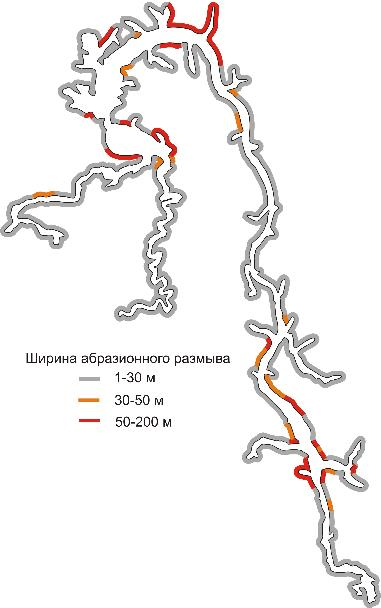
\includegraphics[width=0.8\linewidth]{pics/image13.png}
    \caption{Карта районирования берегов Братского водохранилища по ширине абразионного размыва}
    \label{fig:bratsk-res}
  \end{figure}

Объектом исследования является Братское водохранилище (рисунок~\ref{fig:bratsk-res}). На карте красным цветом выделены участки береговой зоны с высокой интенсивностью абразионного размыва (ширина абразивного размыва 50-200~м).

При долгосрочном прогнозе абразионной переработки берегов Братского водохранилища на 25-летний период эксплуатации, сделанного Г.~И.~Овчинниковым в 90-х годах прошлого века~\cite{ovch99}, максимальные размывы (до 100 м) прогнозировались для участков, сложенных рыхлыми отложениями основной акватории правого берега водоема.
Протяженность берегов Братского водохранилища составляет 6030 км, около 38~\% сложено рыхлыми четвертичными отложениями. Абразионные берега составляют 2056 км (34.2~\% общей протяженности берегов)~\cite{ovch03}. Максимальная ширина размыва характерна для склонов, сложенных рыхлыми образованиями (пески, лессовидные супеси и суглинки), минимальные – для скальных и полускальных грунтов (песчаники, доломиты, известняки, алевролиты, аргиллиты, мергели) (рисунок~\ref{fig:bratsk-res}).

Результаты долговременного мониторинга показали, что после более 50-ти лет эксплуатации Ангарских водохранилищ береговая зона все еще не достигла стадии устойчивого равновесия.  Сохраняется стабильная динамика абразионного размыва, особенно береговых склонов, сложенных рыхлыми отложениями (рисунок~\ref{fig:bratsk-res}).


На рисунке~\ref{fig:water-level} показаны многолетние изменения уровня воды в  водохранилище — основного фактора, вызывающего деградационные геологические процессы, частично находящегося под управлением технологических процессов каскада электростанций Иркутской области.

  \begin{figure}[htp]
	\centering
    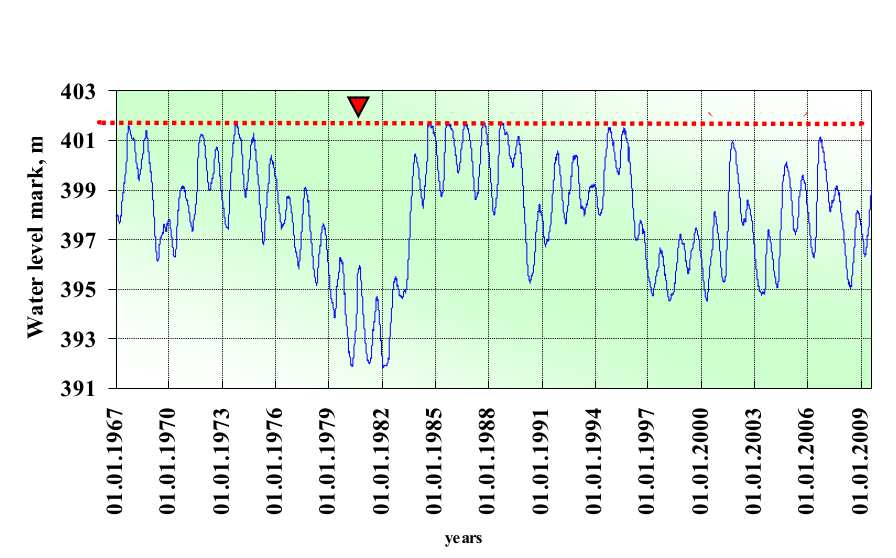
\includegraphics[width=\linewidth]{pics/image17.png}
    \caption{Изменение уровня Братского водохранилища за период 1967-2009 гг (по данным метеостанции Балаганск)}
    \label{fig:water-level}
  \end{figure}

От стабильности береговой зоны зависит возможность ее технического, рекреационного и др. видов использования, особенно в условиях, когда уровень воды регулируется технически в достаточно большом диапазоне значений сезонного (2-3~м) и многолетнего регулирования (до 10~м).

  \begin{figure}[htp]
	\centering
    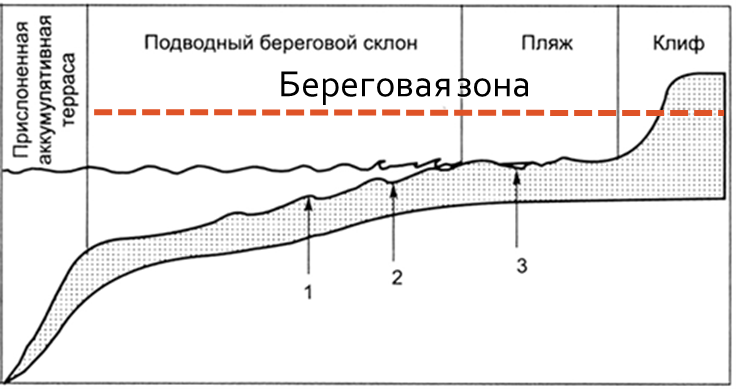
\includegraphics[width=\linewidth]{pics/image1.png}
    \caption{Схема строения береговой зоны водоема}
    \label{fig:shore-schema}
  \end{figure}

За положение береговой линии принята последовательная линейная характеристика - положение бровки берегового уступа, которое изменяется под воздействием волновой деятельности водохранилища и процессов разрушения берегового уступа.

Для формирования политики использования береговой зоны необходимо проводить мониторинг геологических процессов береговой зоны водохранилищ, для этого необходимо проводить каталогизацию и хранение данных, включая исторические данные и современные. До использования спутниковых изображений для получения первичных данных о контуре береговой линии использовались полевые измерения и исследования и аэрофотосъемка. В настоящее время стали доступны съемка со спутника, получение ортофотопланов при помощи квадрокоптеров, измерения ключевых точек при помощи GPS/GLONASS.

Количество данных, таким образом, становится достаточно большим и требует цифрового представления в виде информационной системы, отражающей данные на некоторую координату. В связи с этим одним из важнейших компонентов информационных ресурсов являются геоинформационные системы, поскольку они позволяют согласованно представлять и системно анализировать информацию о географически связанных объектах природной среды и при этом собирать и хранить данные с автоматизированных средств наблюдений и классических средств сбора, осуществлять их автоматизированную обработку и представление в картографическом виде.

Для мониторинга краткосрочной и долгосрочной динамики изменений протяженных побережий в Европе \cite{kabuth14}, странах Юго-Восточной и Южной Азии \cite{isha20},\cite{matin21} применялась DSAS.

\textbf{Цель работы  -- разработать геоинформационную систему крупного водного объекта для мониторинга береговой зоны.}

\paragraph{Задачи}
\begin{enumerate}
\item Проведение полевых исследований (снятие координат),
\item Оцифровка данных береговой линии (координат, спутниковых изображениях, аэрофотоснимков, ортофотопланов),
\item Реализация автоматизации некоторых этапов п.~2 на основе современных технологий,
\item Организация доступа к внешним данным (уровни водохранилища),
\item Прогнозирование динамики береговой зоны,
\item Оценка влияния опасных факторов на технические и социальные объекты в береговой зоне.
\end{enumerate}

Научная новизна разработанных технологий и полученных результатов заключается в использовании новых алгоритмов распознавания объектов на растровых изображениях (линии бровки берегового уступа) при условии ограниченности вычислительных ресурсов и информационного обеспечения.


\subsection*{Автоматизация распознавания береговой линии: обзор технологий}

Фундаментальные исследования уникальных экологических систем, какой является береговая зона крупного водного объекта, проводимые в мире и России, базируются на мониторинге, основывающимся на больших данных. Мониторинг опасных экзогенных геологических процессов входит в единую информационную систему Государственного мониторинга состояния недр, который является составной частью государственного мониторинга состояния и загрязнения окружающей среды. Результаты долговременного мониторинга Братского водохранилища показали, что после более 50-ти лет эксплуатации Ангарских водохранилищ береговая зона все еще не достигла стадии устойчивого равновесия. Разрушение берегов под воздействием природных геологических процессов (абразии, карста, эрозии, оползней) в значительной мере осложняет функционирование береговой зоны. От стабильности береговой зоны зависит возможность ее технического, рекреационного и др. видов использования, особенно в условиях, когда уровень воды регулируется технически в достаточно большом диапазоне значений сезонного (2-3~м) и многолетнего регулирования (до 10~м).

Наборы данных мониторинга характеризуются разнородностью и разноструктурированностью (электронные таблицы, тематические карты, космоснимки, 3D-модели, фото и видеоизображения), пространственно-временной привязкой, большим объемом и высокой скоростью роста объемов информации. Очевидно, что бльшая часть информации, связанной с мониторингом, является неструктурированной, т.е. для ее алгоритмической обработки необходимо решать сложные задачи распознавания ее структуры. Причем вычислиельная сложность данного этапа предварительной обоработки информации является очень высокой.  В данном исследовании рассматривается проблема автоматизированного преобразования растрового представления изменяющегося во времени контура береговой линии равнинного водохранилища в векторный формат для дальнейшего мониторинга геологических процессов.

Аналогичные задачи в настоящее время являются актуальными, причем каждый конкретный случай характеризуется определенной спецификой, связанной с различными характеристиками входных изображений: качество снимков, масштаб бъекта исследования, наличие предварительно обработанных вручную вариантов задач, мощность и сложность вычислительной инфраструктуры. Приведем несколько примеров, найденных в научных статьях. 

В исследовании \cite{b1} предложен подход к поддержке решения задачи выявления и мониторинга береговых линий и оценке эрозии берегов. При помощи спутниковых снимков высокого разрешения территории Вьетнама, использовались модели глубокого обучения. Цели исследования: (1) предложить индикаторы для идентификации береговых линий и берегов; (2) построить модели глубокого обучения (DL) для автоматического дешифрирования береговых линий и берегов по снимкам дистанционного зондирования высокого разрешения; и (3) применить модели, обученные DL, для мониторинга эрозии берегов Вьетнама. Получены восемь DL-моделей на основе четырех вариантов искусственных нейронных сетей, включая U-Net, U2-Net, U-Net3+ и DexiNed. В качестве исходных данных для обучения моделей использовались изображения высокого разрешения, полученные с помощью программы Google Earth Pro. В результате U-сеть, использующая размер входного изображения 512×512, обеспечила наивысшую производительность 98~\% при функции потерь~--~0.16. Результаты интерпретации этой модели использованы для идентификации береговой линии при оценке эрозии берегов из-за повышения уровня моря и штормов в течение 20 лет. Результаты показали, что линия уреза воды идеально подходит для наблюдения за сезонными приливными изменениями или непосредственными движениями волн, то линия бровки подходит для оценки береговой эрозии, вызванной влиянием повышения уровня моря и штормов. Данная работа сформировала отношение к тому, как модель U-Net может быть использована для прогнозирования изменений береговой линий государств, граничащих с мировым океаном.
% The DL models employ preset functions to modify the states of the original input data. Accordingly, the DL architecture for image classification commonly contains six-layer types: INPUT, Convolutional (CONV), Batch Normalization, Pooling, Concatenate, and Dropout layers. The training model analyzes the raw pixel values of all subimages from the INPUT layer (Dang et al., 2020b; Giang et al., 2020). The outputs of neurons are governed by filters in the CONV layers.

Разработка автоматизированной масштабируемой методики выделения береговой линии на основе спутниковых снимков в настоящее время ограничена низкой доступностью открытых, глобально распределенных и разнообразных размеченных данных, на основе которых можно разрабатывать и тестировать методики. В исследовании \cite{b2} представлен Sentinel-2 Water Edges Dataset (SWED), новый и специально разработанный набор маркированных изображений для разработки и тестирования методов автоматического извлечения данных о морфологии береговой линии, используя снимки Sentinel-2. SWED состоит из 16-ти размеченных сцен Sentinel-2 для обучения и 98-ми пар «метка-изображение» для тестирования, данные получены из разных мест мира и содержат примеры большого количества различных типов береговой линии, природных и антропогенных особенностей береговой линии. Для получения оценки качества распознавания для SWED обучены и протестированы четыре модели конволюционных нейронных сетей, основанных на архитектуре U-Net. Модели оптимизированы с использованием категориальной потери перекрестной энтропии, потери Сёренсена-Дайса и двух новых функций потерь, которые используются для фокусировки внимания обучения модели на границе вода-суша. С помощью гибридного процесса количественной и качественной оценки модели показано, что модель, обученная с использованием новой функции потерь Sobel-edge, обладает большей чувствительностью к мелкомасштабным, узким особенностям береговой линии, в то время как количественная производительность, продемонстрированная категориальной перекрестной энтропией, близка к максимальной. Набор данных SWED опубликован в открытом доступе для использования сообществами специалистов по дистанционному зондированию и машинному обучению, а потеря Sobel-edge доступна для использования в приложениях машинного обучения, где важна чувствительность к граничным особенностям.
% SWED is available as free, open data at https://openmldata.ukho.gov.uk.Sentinel-2 Water Edges Dataset  The highest spatial resolution of the Sentinel-2 Multi-Spectral In­ strument (MSI) is 10 m (10 bands)

Статья \cite{b3} рассматривает задачу сегментации морской территории (СМТ) -- важной задачи дистанционного зондирования для различных береговых и экологических исследований, таких как выделение береговой линии, береговая эрозия, мониторинг прибрежных районов, обнаружение судов или айсбергов. Данное исследование направлено на улучшение производительности СМТ путем модификации модели Standard U-Net (SUN) и разработки системы автоматического выделения береговой линии. Модель SUN в целом имеет приемлемые характеристики для многих приложений, но вопросы повышения надежности выделения береговой линии оставются актуальными. В предложенной системе в первую очередь анализируются три различных входных изображения: красно-зелено-синие (RGB), нормализованный индекс разности воды (NDWI) и изображения ближнего инфракрасного диапазона (NIR).  Затем для улучшения результатов сегментации в архитектуру SUN внесены изменения. Основные модификации заключаются в использовании различных функций потерь и двух методов слияния для RGB- и NIR-изображений. Результаты сегментации переданы в последующий конвейер автоматического выделения береговой линии на основе морфологических операций и анализа связности пикселей. Этапы обучения и тестирования выполнены на основе эталонного набора данных о прибрежных районах Китая. Кроме того, для оценки эффективности алгоритмов собран дополнительный набор данных, состоящий из временного ряда снимков Landsat-8 Южного побережья Каспийского моря. Результаты показывают, что предложенные изменения эффективно повышают производительность SUN, при этом наиболее значительное улучшение показателя <<пересечения над объединением>> (IoU), значение которого достигает 1,68\% и 8,95\% в наборах данных Китая и Каспийского моря, соответственно, а также превосходит другие современные модели, включая FC-DenseNet и DeepLabV3+.

Таким образом, современные средства \cite{b1}-\cite{b3} автоматизации построения контуров береговых линий строятся с использованием нейронных сетей (НС) глубокого обучения, получаемых, в некоторых случаях, при помощи дообучения. Процесс обучения организуется на основе большого количества размеченных спутниковых изображений, разметка делается вручную, что достаточно трудоемко. Применяемый в данной ВКР подход основывается на использовании предобученной НС Segment Anything (SA), распознающей предметы (порядка миллиона классов) на изображении. SA не обучалась на распознавание береговых линий, но тестовые испытания показали хорошие результаты выделения контуров областей, граничащих с береговой линией. Чтобы определить контур, необходимо распознать объекты, включающие точки контура. Для этого необходимо провести процесс распознавания, с использованием дополнительной эвристической информатизации.

Процесс распознавания контура реализуется пошагово: 1) в ГИС (геоинформационной системе) выбирается интересующая область и контур береговой линии с векторной карты OpenStreetMap, данный контур является начальным приближением результата; 2) для выбранной области с серверов дистанционного зондирования загружаются изображения с разметкой по конкретным датам, изображения помещаются в серверное хранилище; 3) запуск системы SegmentAnything в режиме распознавания всех возможных объектов, результат распознавания в виде набора бинарных масок сохраняется на сервере; 4) алгоритмический анализ свойств объектов, представленных масками, и их расположение относительно друг друга и краёв изображения, результаты сохраняются в А-боксе онтологии на сервере; 5) анализ взаимного расположения объектов, выявление множества точек, относящихся к береговой линии; 6) построение контура по выявленным точкам (перевод в векторный формат), сохранение результата в shape-файл.

Преимущества предложенного подхода -- это а) отсутствие трудоемкого этапа подготовки данных для обучения НС, б) распознавание контура представляется (программируется) в виде правил, что дает возможность управлять процессом распознавания, в частности <<сцеплять>> объекты или контуры с разных изображений; в) SA, ввиду обученности на большом количестве изображений не привязана к свойствам конкретных изображений (размеру, цветовой гамме, повороту и т.д.), что позволяет г) реализовывать (в перспективе) процедуры последовательного уточнения характеристик береговой линии, переходя к изображениям более высокого разрешения.

\chapter{Методики прогнозирования состояния береговой зоны}\label{chap:techniques}

Прогнозирование изменений геологической среды является одним из приоритетных научных и прикладных направлений в науках о Земле. Мониторинговые исследования за изменениями природно-технических систем и их отдельных элементов являются надежной базой для прогнозных оценок.

В 1972 году на Стокгольмской конференции ООН Р. Манном впервые было введено понятие глобального мониторинга окружающей среды (global environmental monitoring system — GEMS), которым он обозначил систему повторных наблюдений окружающей среды в пространстве и времени. С этого момента термин «мониторинг» вошел в нашу научную литературу и стал применяться в разных областях знаний, в том числе и в области геологии~\cite{ivanov01}. В области инженерной геологии стационарные наблюдения сопутствовали инженерным изысканиям на всех сложных объектах. Первая оползневая станция ЦНИГРИ в Крыму была организована в 1930 году.

Для Ангарского каскада ГЭС лабораторией инженерной геологии и геоэкологии ИЗК СО РАН была создана система геодинамических полигонов и стационаров, расположенных в различных ландшафтных условиях. Систематические ежегодные наблюдения за отдельными видами ЭГП проводились на 77 участках, среди которых на 43 изучалась абразия, на 15 -- гравитационные процессы, на 11 -- карстово-суффозионные и на 8 -- эрозионные~\cite{koz18}.

Целью мониторинговых исследований является изучение режима и условий функционирования локальных береговых геосистем и их изменения под воздействием техногенных факторов, связанных с созданием и режимом эксплуатации водохранилища.

В нашей стране наиболее применяемыми в настоящее время являются методы, предложенные Е. Г. Качугиным (1959), Г. С. Золотаревым (1969), Н. Е. Кондратьевым (1960), Е. К. Гречищевым (1961) Л. Б. Розовским, И. П. Зелинским (1975), И. А. Печеркиным (1969), Институтом земной коры СО РАН (1976 г.), ПНИИСом (Рагозин и Бурова, 1993) и другими научными коллективами.
По различным критериям все виды прогнозов переработки берегов водохранилищ могут быть объединены в три разных класса (рисунок~\ref{fig:prognosys-schema})~\cite{ivanov01}. Так, временные прогнозы подразделяются на краткосрочные (предупредительные) с периодами прогнозирования от 1 до 10 лет и долгосрочные (перспективные), включающие прогнозы на 10 и более лет, в том числе на конечную стадию развития берега. Пространственные прогнозы объединяют в себе локальные, ха­рактеризующие переработку по отдельным профилем (профильный прогноз) или участкам (площадной прогноз) и выполняемые в масштабах 1:1~000—1; 10~000; и региональные, характеризующие переработку по периметру всего водохранилища или его отдель­ной части и производимые в масштабах 1:25~000—1:200~000. По теоретическим предпосылкам обоснования расчетов все методы подразделяются на три группы — энергетические, геологического подобия и вероятностно-статистические (или стохастические, по Г. С. Золотареву (1990)).

  \begin{figure}[htp]
	\begin{center}
	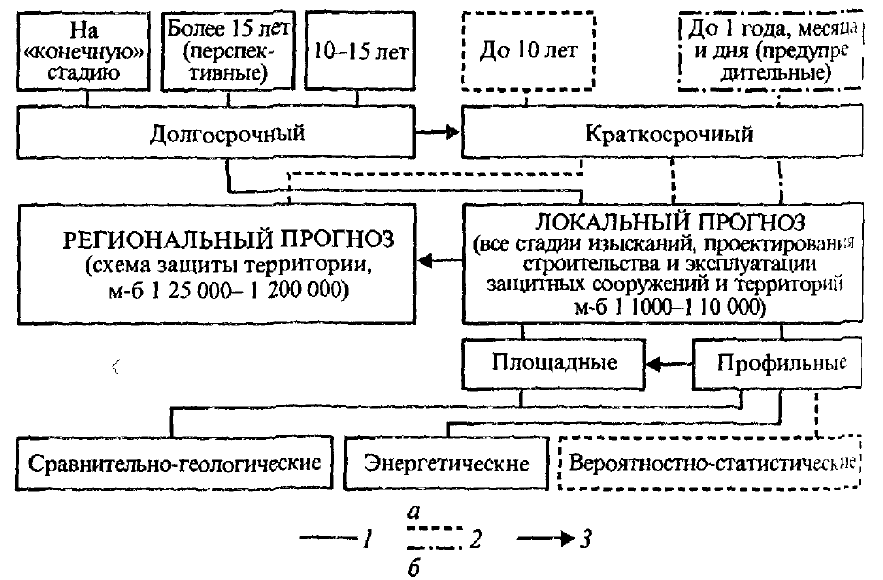
\includegraphics[width=0.8\linewidth]{pics/image4.png}
  \end{center}
  \begin{quote}  
    Прогнозы, выполняемые на водохранилищах: 1 — проектируемых и эксплуатируемых; 2 — эксплуатируемых: а — на всех стадиях изысканий и проектирования инженерной защиты, б — в процессе строительства и эксплуатации; 3 — последователность выполнения прогнозов.
  \end{quote}
  \caption{Схема прогнозов процессов переработки берегов водохранилищ при инженерных изысканиях для освоения и защиты прибрежные территорий~\cite{rec86}}
    \label{fig:prognosys-schema}
  \end{figure}

В научно-технической литературе известны три группы методов прогнозной оценки переработки берегов водохранилищ:
\begin{enumerate}
\item энергетические (\cite{b22}, \cite{b23} и др.);
\item сравнительно-геологические (\cite{b18}, \cite{b19} и др.);
\item вероятностно-статистические \cite{b20}.
\end{enumerate}

\textbf{Энергетические методы} при прогнозе преимущественно учитывают энергию волнения (гидрологический фактор), область применения их ограничена простыми и однородными в инженерно-геологическом отношении условиями, характеризуются низкой точностью прогнозной оценки. Для их обоснования требуются значительные трудозатраты по каждому расчетному поперечнику. Применимы только на первой стадии переработки берегов действующих водохранилищ.

\textbf{Сравнительно-геологические методы}  основаны на аналогиях природно-техногенных условий водохранилищ. Основные трудности, снижающие точность прогнозных оценок в этих методах связаны с подбором надежных аналогов и выбором критериев подобия, что редко удается сделать в реальных условиях.

\textbf{Метод вероятностно-стохастических моделей}~\cite{b20} по своей технической сущности наиболее близок к предлагаемому техническому решению (прототип). Этот метод заключается в учете зависимостей переработки берегов от различных природно-техногенных факторов по данным режимных наблюдений с построением стохастических моделей процесса. Его основной недостаток, несмотря на большие трудозатраты снижающий точность прогнозной оценки, заключается в недоучете общих закономерностей развития процесса, стадийности формирования берегов, требует большого объема режимных наблюдений по каждому расчетному поперечнику в отдельности.

В Институте земной коры СО РАН Е. К. Гречищевым (1961). был разработан энергетический метод, позволяющий производить прогноз ширины зоны размыва на разное количество лет. Для прогноза необходимы сведения по ветровому волнению, определяющему энергию, знание уровенного режима водоемов, точные инженерно-геологические разрезы по расчетным профи­лям и данные по размываемости грунтов. Ширина зоны размыва определяется через объем раз­мытых горных пород.

Позже по результатам исследований динамики берегов водохранилищ Ангарского каскада ГЭС и выявленных закономерностей развития береговой зоны был сделан прогноз размыва берегов на 25-летнюю стадию развития~\cite{ovch99}. Расчеты производились по методике, разработанной в Институте земной коры СО РАН, учитывающей весь спектр факторов (геолого-геоморфологические, морфометрические, гидродинамические и техногенные), влияющих на динамику берегов. Кроме того, использовались прогнозно-диагностические модели динамики берегов, построенные на основе многолетних рядов наблюдений по стационарным участкам, расположенным в различных геолого-геоморфологических и гидродинамических условиях. Учет влияния колебания уровня воды в водохранилищах оценивался его повторяемостью на определенных отметках в пределах выделенных полутораметровых подзон. Прогноз был выполнен с учетом того, что в 50 \% случаев уровень воды будет находиться в пределах верхней подзоны размыва.

\section{Геоинформационные системы}


\emph{Геоинформационные системы (ГИС)} - это автоматизированные системы, функциями которых являются сбор, хранение, интеграция, анализ и графическая интерпретация пространственно-временных данных, а также связанной с ними атрибутивной информации о представленных в ГИС объектах.

\textbf{Классификация ГИС~\cite{gisclass}}.
Географические информационные системы классифицируют по-разному в зависимости от масштабности и функционала, а также других признаков.

По территориальному охвату ГИС бывают:
\begin{itemize}
\item глобальными;
\item субконтинентальными;
\item национальными;
\item региональными;
\item субрегиональными;
\item локальными или местными.
\end{itemize}

По уровню управления:
\begin{itemize}
\item федеральными;
\item региональными;
\item муниципальными;
\item корпоративными.
\end{itemize}

По функциональности:
\begin{itemize}
\item полнофункциональными;
\item для просмотра данных;
\item для ввода и обработки данных;
\item специализированными с дополнительными функциями.
\end{itemize}

По предметной области:
\begin{itemize}
\item картографическими;
\item геологическими;
\item городскими или муниципальными;
\item природоохранными,
\item туристическими.
\end{itemize}

Если в ГИС присутствуют возможности цифровой обработки изображений, то такие системы называются интегрированными ГИС (ИГИС). Полимасштабные, или масштабно-независимые ГИС обеспечивают графическое или картографическое воспроизведение данных в любом масштабе с наибольшим разрешением. Пространственно-временные ГИС работают с данными во времени.

\textbf{Предметом исследования ВКР} является процесс сбора данных и построения прогноза изменения береговой линии водохранилища.

Для обеспечения оценки состояния береговой зоны и ее перспективного состояния может быть оценено при помощи получения дополнительных данных в результате математического моделирования. Процесс размывания/накопления грунта зависит от комплекса природных и внешних факторов таких как:
\begin{itemize}
\item Положение и продолжительность стояния уровня водохранилища;
\item Геолого-геоморфологические условия строения  береговой зоны;
\item Ветро-волновая нагрузка на участке берега размыва.
\end{itemize}

Самым точным емким  информационным подходом является моделирование процесса размыва как физического процесса. Такой подход требует большое количество данных и построение сложных алгоритмов моделирования, а также много вычислительных ресурсов. В результате получается краткосрочный прогноз.

В данной работе использована модель грубой оценки контура береговой линии на основе проведения экстраполяции при помощи метода, реализованного в библиотеке DSAS\cite{isha20}, реализованной в виде модуля ArcGIS. Исходный код является открытым и представлен на языке C\#.

Digital Shoreline Analysis System (DSAS) DSAS v5.0 - это модуль для ArcGIS 10, разработанный совместно Геологической службой США (USGS) и TPMC Environmental Services~\cite{himmel09}, \cite{himmel18}. Разработанный алгоритм данного программного обеспечения позволяет пользователю вычислить скорость изменения береговой линии, используя географически привязанные береговые линии временных рядов в каждом разрезе с заданным пользователем временным интервалом.

DSAS использует пять операций, в частности, огибающую изменения береговой линии (shoreline change envelope SCE), чистое движение береговой линии (net shoreline movement NSM), скорость конечной точки (end point rate EPR), скорость линейной регрессии (linear regression rate LRR) и наименьшую медиану квадратов (least median of squares LMS) для оценки скорости изменения береговой линии в долгосрочной и краткосрочной перспективе.

За положение береговой линии принимается любая, указанная пользователем, линейная характеристика, такая как линия растительности, линия высокой воды, линия низкой воды или линия влажности/сухости. В данном случае за положение береговой линии принимается положение бровки берегового уступа, которое изменяется под воздействием волновой деятельности водохранилища и процессов разрушения берегового уступа.

\begin{itemize}
\item Прогноз DSAS смотрится при помощи экстраполяции точек контура, исходя из данных о контурах линий, соответствующих определенным датам съемки. Подход обладает рядом преимуществ:
\item   Не требует больших вычислительных ресурсов,
\item   Не требует данных о конкретных геологических процессах,
\item   Прост в реализации,
\item   Для модели не требуется большое количество данных,
\item   Данные могут охватывать большие диапазоны дат,
\item   Реализует прогноз на далекую перспективу,
\item   Случайные техногенные воздействия “усредняются” повторяющимися постоянными природными факторами.
\end{itemize}

К недостаткам модели относятся следущие:

\begin{itemize}
\item Модель дает достаточно грубую оценку расположения контура береговой линии,
\item Достаточно сложно использовать при наличии периодически меняющихся факторов воздействия (см. например, проблематику моделирования уровня Каспийского озера).
\end{itemize}
Факторы воздействия на береговую линию Братского водохранилища характеризуются комплексностью, одним из которых является антропогенность, а именно, уровень воды. 

Береговые линии могут быть оцифрованы из различных источников (например, цифровые ортофотопланы, привязанные исторические карты береговой съемки или спутниковые снимки), собраны с помощью полевых исследований с глобальной системой позиционирования или извлечены из лидарных исследований. Приведем примеры исходных данных. На рисунке~\ref{fig:google-src} представлены два варианта: а) точки контура бровки, отснятые в поле (2008 год) и б) изображение берега, полученное с серверов Google Maps.

\begin{figure}[htp]
  \centering
  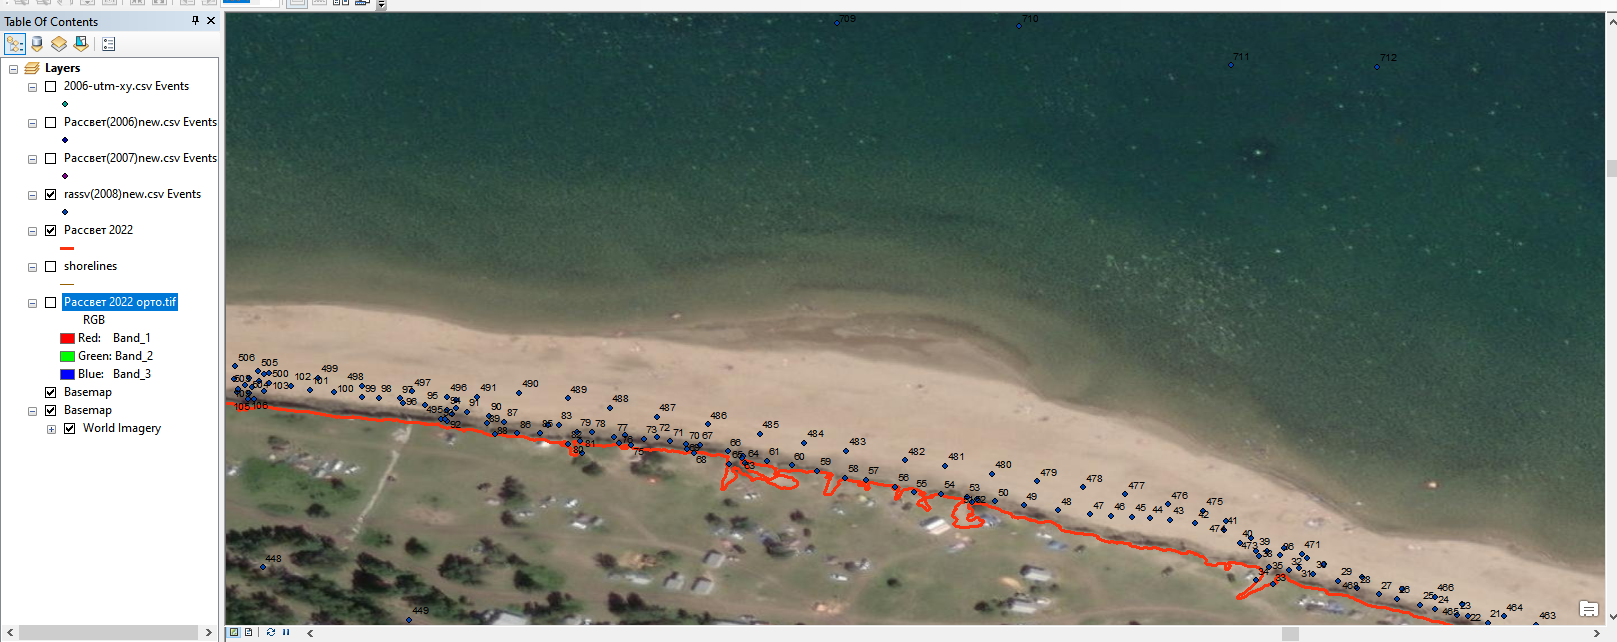
\includegraphics[width=\linewidth]{pics/image22.png}\label{fig:google-src}
  \caption{Контур береговой линии представлен координатами точек и изображением с сервера}
\end{figure}

Более точными исходными данными являются спутниковые снимки высокого разрешения и отснятые и обработанные изображения, полученные при помощи квадрокоптера (ортофотопланы). Сервера спутниковых снимков высокого разрешения позволяют также получать информацию не только для текущего года, но и за предыдущие года, однако их достаточно трудно получить ввиду их частичной открытости. Ортофотопланы (рисунок~\ref{fig:ortho-src}) можно снимать каждый год, они дают приемленое разрешение, а также для осуществления съемки не требуется дольших материальных затрат.

\begin{figure}[htp]
  \centering
  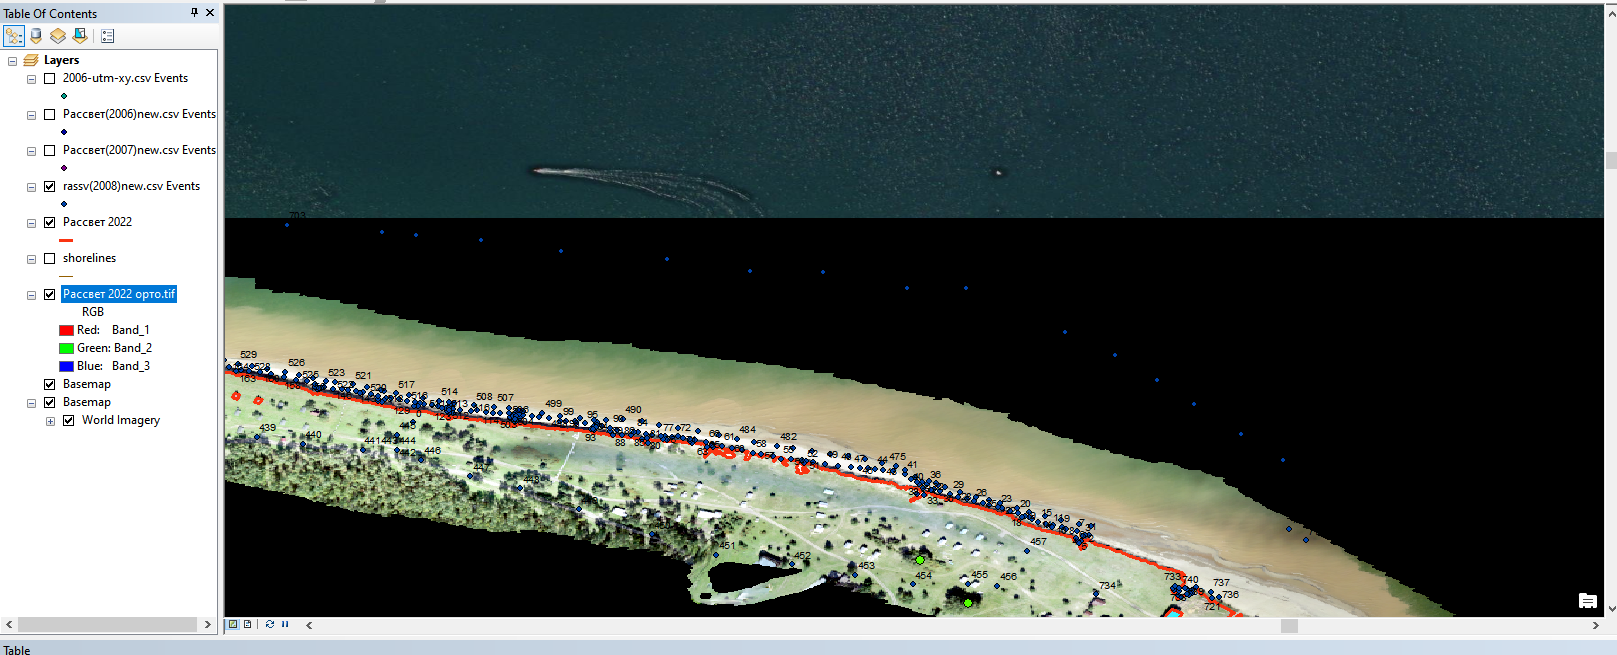
\includegraphics[width=\linewidth]{pics/image12.png}\label{fig:ortho-src}
  \caption{Контур береговой линии представлен координатами точек и изображением с сервера}
\end{figure}

Каждый вектор береговой линии представляет собой определенное положение во времени и имеет дату в таблице атрибутов класса характеристик береговой линии (таблица~\ref{tbl:struct}). Измерительные трансекты, откладываемые DSAS от базовой линии, пересекают векторы береговой линии (рисунок~\ref{fig:dsas-trans}). Точки пересечения предоставляют информацию о местоположении и времени, используемую для расчета скорости изменения. Расстояния от базовой линии до каждой точки пересечения вдоль трансекты используются для расчета выбранных статистических данных.

\begin{table}
  \caption{Атрибуты шейп-файла shorelines для Digital Shoreline Analysis System (DSAS) version 5.0}\label{tbl:struct}
  \centering
  \begin{tabular}{|l|l|l|}
    \hline 
    Field name &	Data type &	Attribute addition\\\hline 
    OBJECTID	& Object ID	& Autogenerated\\
    SHAPE & 	Geometry	& Autogenerated\\
    SHAPE Length	& Double	& Autogenerated\\
    DATE	& Text (Length=10 OR Length=20)& User-created	\\
    UNCERTAINTY	& &	User-created	\\
    SHORELINE\_TYPE	& &	User-created\\
    \hline
  \end{tabular}
\end{table}

\begin{figure}[htp]
  \centering
  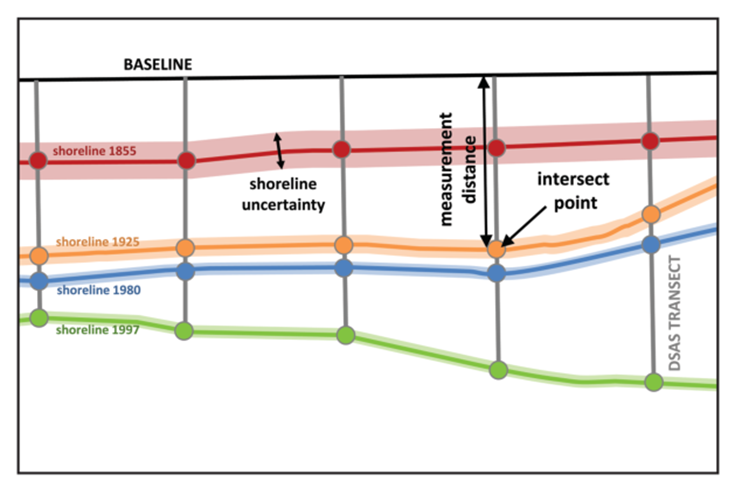
\includegraphics[width=\linewidth]{pics/image9.png}\label{fig:dsas-trans}
  \caption{Трансекты DSAS}
\end{figure}

В связи с вышеперечисленным применение именно этой модели позволит сделать первый шаг в построении системы поддержки принятия решения о характере деградационных процессов береговой зоны, и, таким образом, поможет представить необходимую информацию муниципальному хозяйству данные о политике использования того или иного берега.

Как было сказано ранее одной из проблем использования математического моделирования - это информационное обеспечение, т.е. создание возможности подачи исходных данных в процесс моделирования. Для применения DSAS необходимо представить набор файлов требуемой структуры - Shapefile с контурами береговых линий, и соответствующий ему файл данных - значения атрибутов. Контуры и атрибуты могут быть получены при помощи привязки и оцифровки контуров в авиа- и спутниковых снимков. Процедура оцифровки достаточно трудоёмкая, и в данной ВКР предлагается подход к ее частичной автоматизации на основе анализа результатов приложения современных методов распознавания объектов на изображении.

\section{Технологии ГИС}

Преимущество ГИС в том, что эта система позволяет преодолеть основные недостатки обычных карт - их статичность и ограниченную емкость как носителя информации. В последние десятилетия бумажные карты из-за перегруженности информацией становятся нечитабельными. ГИС же обеспечивает управление визуализацией информации. ГИС в отличие от других информационно-аналитических систем предназначена для обрабатки и анализа пространственных данных. Информация об этих пространственных данных в цифровой форме называется геоинформацией.

Таматически спецмализированная прикладная ГИС включает в себя пять ключевых составляющих: аппаратные средства, программное обеспечение, данные, исполнители и методы. ГИС-приложения объединяют различные типы информации, среди которых: картографические данные — представлены в виде карты и могут включать такую информацию, как расположение рек, дорог, жилых и нежилых строений; аэрофотоснимки и обычные фотографии и данные со спутников; данные дистанционного зондирования (обычно с применением воздушных шаров и дронов); глобальные системы позиционирования (GPS);данные из Интернета; документы, включая архивные таблицы и каталоги координат; данные из других

  \begin{figure}[htp]
	\centering
	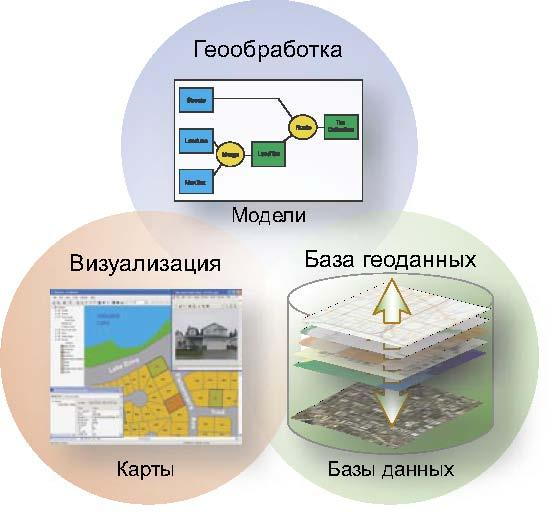
\includegraphics[width=0.7\linewidth]{pics/image15.png}
    \caption{Процесс создания ГИС}
    \label{fig:gis-design-process}
  \end{figure}

Технология ГИС позволяет накладывать все типы информации, независимо от их источника или исходного формата, поверх друг друга на одной карте. ГИС использует местоположение в качестве ключевой переменной, чтобы связать эти, казалось бы, несвязанные данные.
Ввод информации в ГИС называется сбором данных. Информацию, которая уже находится в цифровой форме, можно просто загрузить в систему. Однако сначала карту необходимо отсканировать или преобразовать в цифровой формат (оцифровка данных).

Географические информационные системы включают три компонента:

\textbf{Данные:} ГИС хранит данные о местоположении в виде слоев информации по разным темам. Каждый набор данных имеет таблицу атрибутов, в которой хранится информация об объекте. Два основных типа формата файлов ГИС — растровый и векторный. Растровый представляет собой сетки из ячеек или пикселей. Он полезен для хранения различных ГИС-данных. Векторный формат выглядит как многоугольник, в котором используются точки (называемые узлами) и линии. Векторные файлы нужны для хранения данных ГИС с четкими границами, такими как городские округа или улицы. В итоге технология позволяет отображать пространственные и линейные зависимости. Пространственные показывают топографию местности (поля, ручьи), а линейные представлены дорогами или коммунальными сетями.

\textbf{Аппаратный компонент}, который запускает программное обеспечение ГИС. Это может быть что угодно: мощные серверы, мобильные телефоны или персональные рабочие станции. Как правило, в работе с ГИС нужны два монитора, дополнительное хранилище данных и графические карты высокой четкости.

\textbf{Программное обеспечение}. Оно специализируется на пространственном анализе с использованием математики в картах. Такое ПО сочетает в себе географию с современными технологиями для измерения, количественной оценки и анализа. В ГИС. обычно используют языки программирования Python, SQL, C ++, Visual Basic и JavaScript.

В ГИС информация со всех различных карт и источников должна соответствовать одному масштабу — соотношению между расстоянием на карте и фактическим расстоянием на Земле. При этом разные карты имеют разные проекции. Чтобы перенести изогнутую трехмерную форму на плоскую поверхность, неизбежно требуется растяжение одних частей и сжатие других. Так, на карте мира могут быть показаны либо страны правильного размера, либо их правильные формы, но нельзя отобразить эту информацию одновременно. ГИС берет данные с разных карт мира и объединяет ее, чтобы отобразить в одной общей проекции. Одними из популярных программ ГИС считаются ArcGIS и QGIS.

\chapter{Проектирование ГИС для прогнозирования береговой зоны}\label{chap:proj}

Анализ предметной области, представленный в Главе~\ref{chap:techniques}, показал, что для получения качественно новых результатов научных исследований в инженерной геологии береговых зон внутренних водоемов, необходимо создать ресурсы хранения, преобразования, обеспечения эффективного доступа к этой информации, а также ее визуализации. Перечисленным свойствам удовлетворяют программные системы, называемые \emph{информационными системами} (ИС). Наличие пространственной привязки данных, т.е. ассоциирование конкретной информации с точкой или каким-то объектом на поверхности Земли, переводит ИС в класс \emph{географических информационных систем}. Если элементы (\emph{функциональные блоки}) ИС исполняются на отдельных вычислительных узлах или узлах хранения данных локальной вычислительной сети, и даже в отдельных процессах одного вычислительного устройства, то какая ИС относится к классу \emph{распределенных информационных систем} (\emph{распределенных программных комплексов}), а совокупность сетевых ресурсов, вовлеченных в информационно-вычислительные процессы называется \emph{информационно-вычислительной инфраструктурой} (ИВИ).

В настоящее время элементы ИВИ представляют в виде сервисов, т.е. функциональных блоков, выполняющих заданные операции, получая исходные данные из сети (с другого сервиса) по определенному протоколу, и отправляющие результат также в сеть (на другой сервис). Экстремальным вариантом сервисной ИВИ является так называемая \emph{микросервисная архитектура}. Набор реализуемых функций в таких сервисах минимизирован, и распределенный программный комплекс реализуется композицией большого числа таких микросервисов, сконфигурированных согласно дизайну ИВИ. Преимуществом такого подхода является б\'ольшый потенциал к повторному использованию кода, поддержка стандартизации между отдельными проектами, более гибкой интеграции с другими ИВИ. Кроме того, функционирование процессов микросервисов, как правило, более предсказуемо, что дает возможность более надежного и качественного управления ИВИ.

При проектировании ИВИ решается задача управления распределенным вычислительным процессом -- \emph{синхронизацией} работы \emph{сервисов}. Стандартный способ синхронизации работы сервисов в ИВИ -- это использование специальных сервисов, называемых \emph{брокеров сообщений} (\emph{message brockers}). Брокеры сообщений позволяют конфигурировать ИВИ и управлять этой средой таким образом, чтобы логика вычислительного процесса соответствовала реализуемому алгоритму обработки данных. Также этот сервис обеспечивает перезапуск процессов в ИВИ в случае перезапуска узлов и локальной вычислительной сети. Еще одна функция - это распределение и, в некоторых случаях, перераспределение, балансировка вычислительной нагрузки между узлами, реализующими один и тот же сервис.

Таким образом, представленные в Главе~\ref{chap:techniques} проблемы решаются при помощи реализации распределенной вычислительной среды обеспечения сервисов хранения и обработки данных, где некоторыми функциональными блоками выступают геоинформационные системы.

Таким образом, для обеспечения возможности проведения научных исследований в области инженерной геологии береговых зон водохранилищ необходимо создать ресурсы хранения информации и вычислительные ресурсы, обеспечивающие продуктивную среду прогнозирования с использованием различных математических моделей. Перспективные, в смысле реализации в такой среде, ранжируются по видан задач, масштабу исследуемого объекта, размеру интервала времени, степени точности.

\section{Концептуальная модель предметной области}

Основная цель исследований, в рамках которых получены результаты данной ВКР, заключается в создании системы поддержки принятия решения (СППР) об оценке состояния береговой зоны водохранилищ, включая опасные геологические процессы. СППР, реализуемые с использванием функциональных блоков моделирования и автоматизированной оценки результатов, формирует базу создания \emph{систем поддержки принятия решений} автоматизации выработки \emph{антиинтуитивных решений}\footnote{Антиинтуитивные решения принимаются на основе анализа имеющейся информации, а не на основе интуиции лица, принимающего решения}.

Процесс принятия решений опирается на концептуальное моделирование предметной области. В настоящее время стандартным методом представления концептуальных моделей являются онтологии, явные спецификации концептуального уровня представления предметной области~\cite{gruber}.

Спроектированная онтология (рисунки\ref{fig:ontology-graph},~\ref{fig:xdot}), описывает предметную область инженерной геологии, связанную с развитием и мониторингом экзогенных процессов на берегах водохранилищ. Водохранилища являются искусственно созданными водоемами в отличие от озер. После их создания (в результат строительства ГЭС на реках) на берегах стали активно развиваться экзогенные процессы. На отдельных участках берега исследователи изучают формы экзогенных процессов (воронка, овраг, оползень, эоловая форма), геоморфологические и геологические условия их развития. Для каждого участка определены координаты (latitude, longitude, протяженность в метрах). В зависимости от преобладающих процессов можно определить генетический тип берега. Онтология содержит: 34 класса (рисунок~\ref{fig:onto-classes}), 24 свойств и 21 индивидуумов (рисунок~\ref{fig:bykovo-instance}). Свойства включают примитивные (data property) – 13 (рисунок~\ref{fig:data-props}) и объектные (object property) – 11 (рисунок~\ref{fig:obj-prop-results}).

  \begin{figure}[htp]
	\centering
	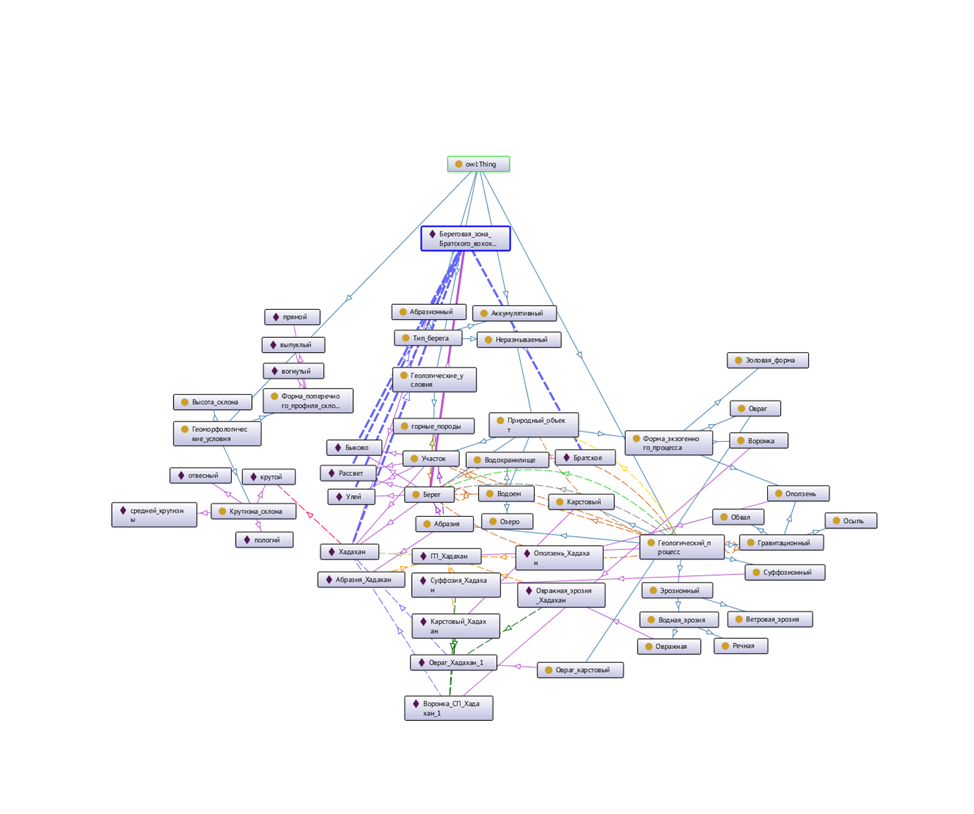
\includegraphics[width=\linewidth]{pics/image6.png}
    \caption{Скриншот экрана с созданной онтологией в OntoGraph}
    \label{fig:}
  \end{figure}

  \begin{figure}[htp]
	\centering
	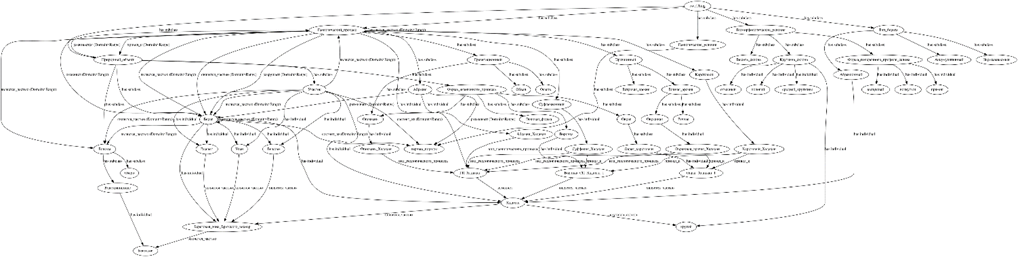
\includegraphics[width=\linewidth]{pics/image3.png}
    \caption{Графическое изображение созданной онтологии, построенная в программе xdot}
    \label{fig:xdot}
  \end{figure}

  \begin{figure}[htp]
	\centering
	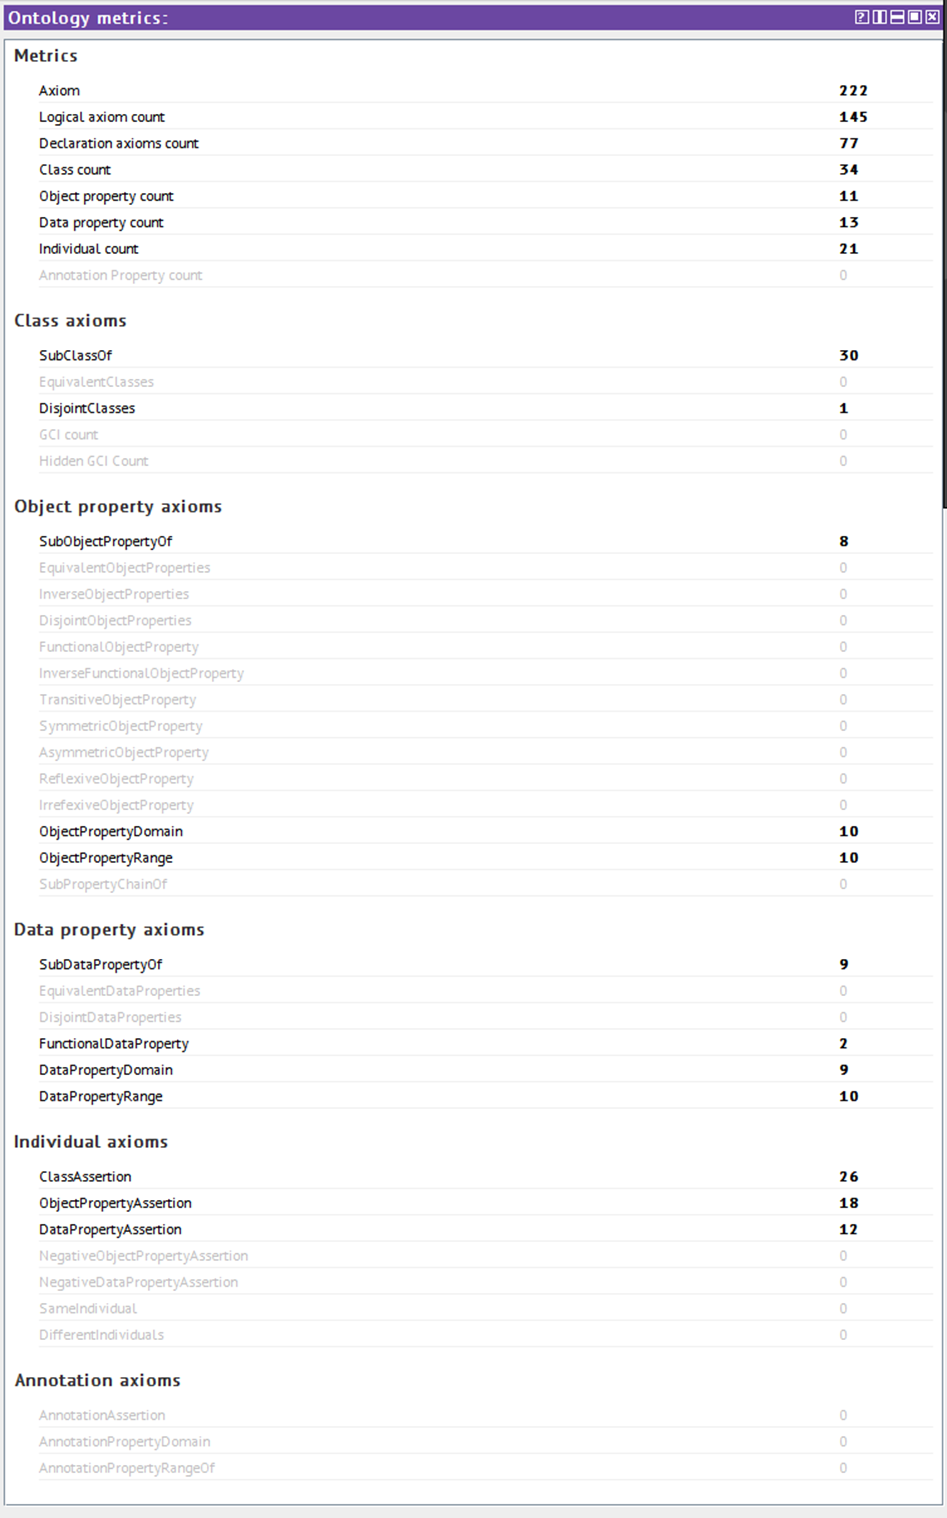
\includegraphics[width=0.7\linewidth]{pics/image21.png}
    \caption{Скриншот панели <<Ontology metrics>>}
    \label{fig:panel-screen}
  \end{figure}


  \begin{figure}[htp]
	\centering
	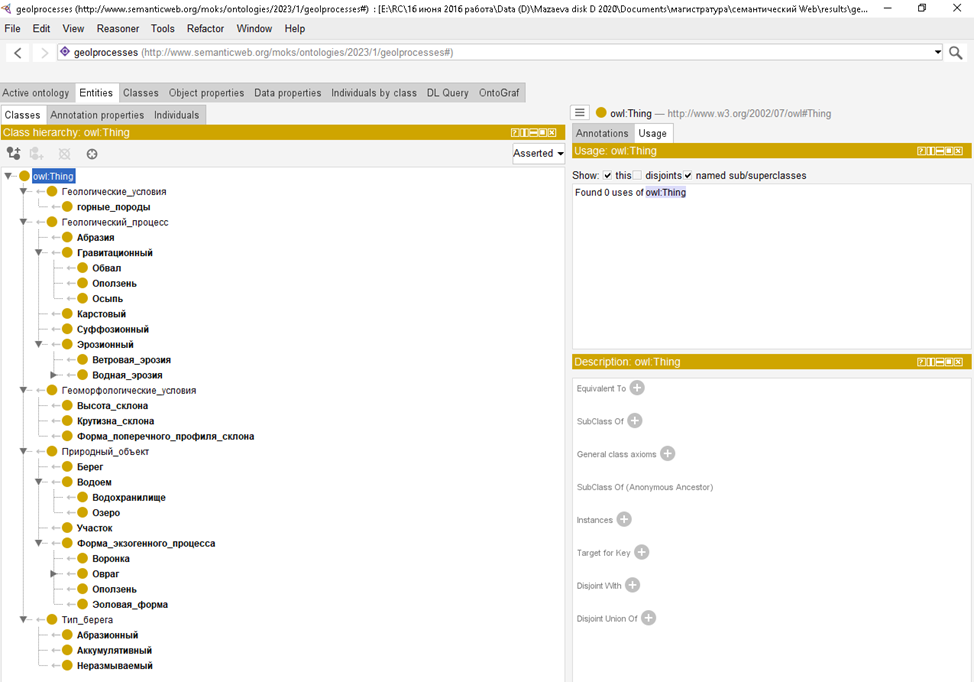
\includegraphics[width=0.9\linewidth]{pics/image16.png}
    \caption{Скриншот экрана с вкладками созданных классов}
    \label{fig:onto-classes}
  \end{figure}

К важным терминам предметной области относятся термины:
\begin{itemize}
\item природный объект;
\item водоем;
\item берег;
\item участок;
\item форма экзогенного процесса.
\end{itemize}
Их иерархия показана на рисунке~\ref{fig:onto-hierarchy}.

  \begin{figure}[htp]
	\centering
	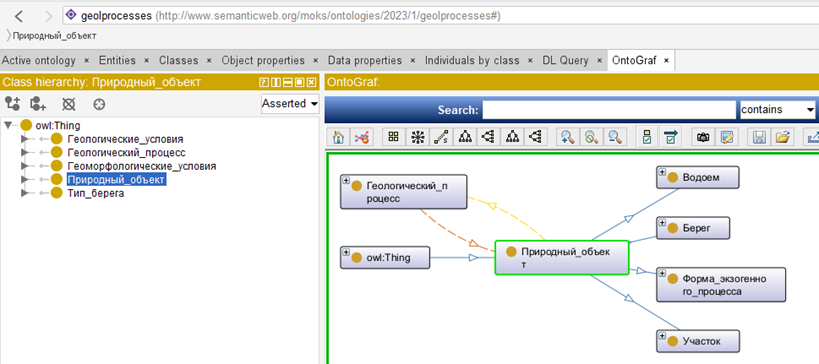
\includegraphics[width=0.9\linewidth]{pics/image2.png}
    \caption{Иерархия важных предметных терминов и ее отображение в OntoGraph}
    \label{fig:onto-hierarchy}
  \end{figure}

Далее представлены скриншоты экранных форм с вкладками созданных свойств и индивидуумов (рисунок~\ref{fig:data-props}.

  \begin{figure}[htp]
	\centering
	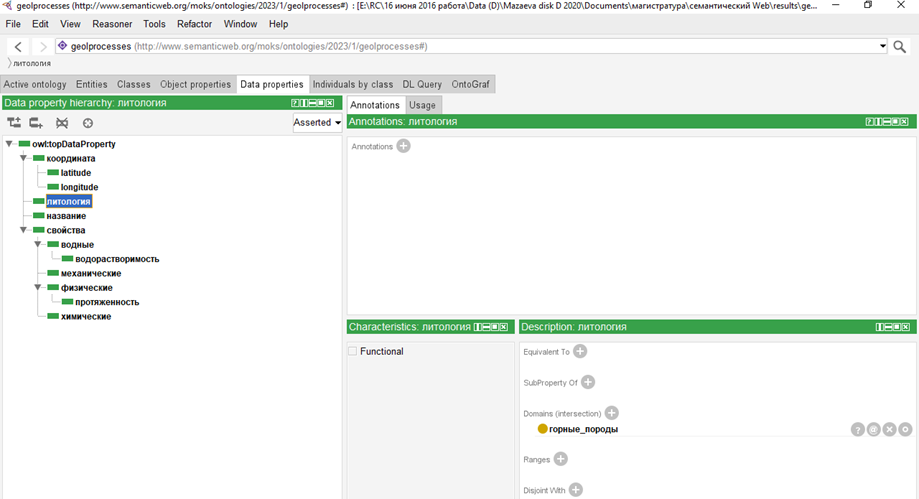
\includegraphics[width=0.9\linewidth]{pics/image24.png}
    \caption{Скриншот экрана панели <<Data properties>> с параметрами свойства для Литология}
    \label{fig:data-props}
  \end{figure}

  \begin{figure}[htp]
	\centering
	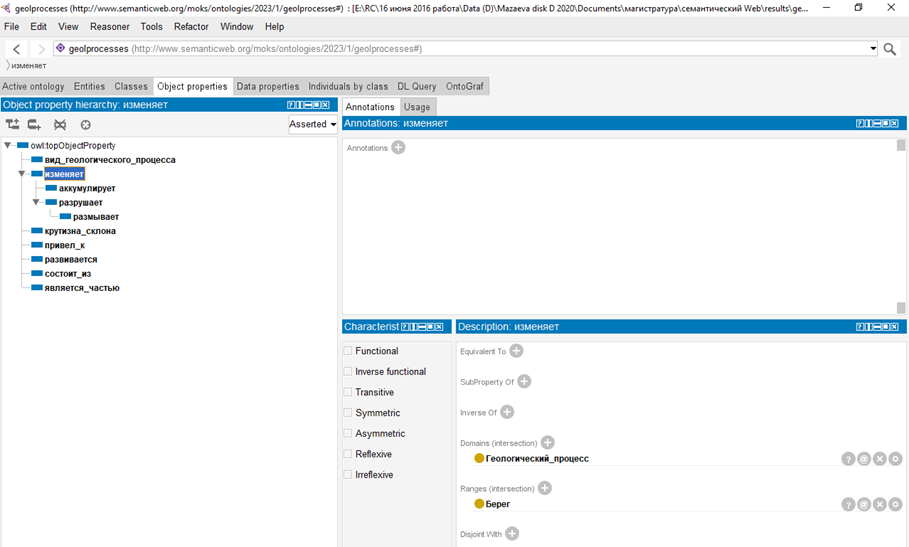
\includegraphics[width=0.9\linewidth]{pics/image10.png}
    \caption{Скриншот экрана панели <<Object properties>> с параметрами свойства для «изменяет»}
    \label{fig:obj-props}
  \end{figure}

  \begin{figure}[htp]
	\centering
	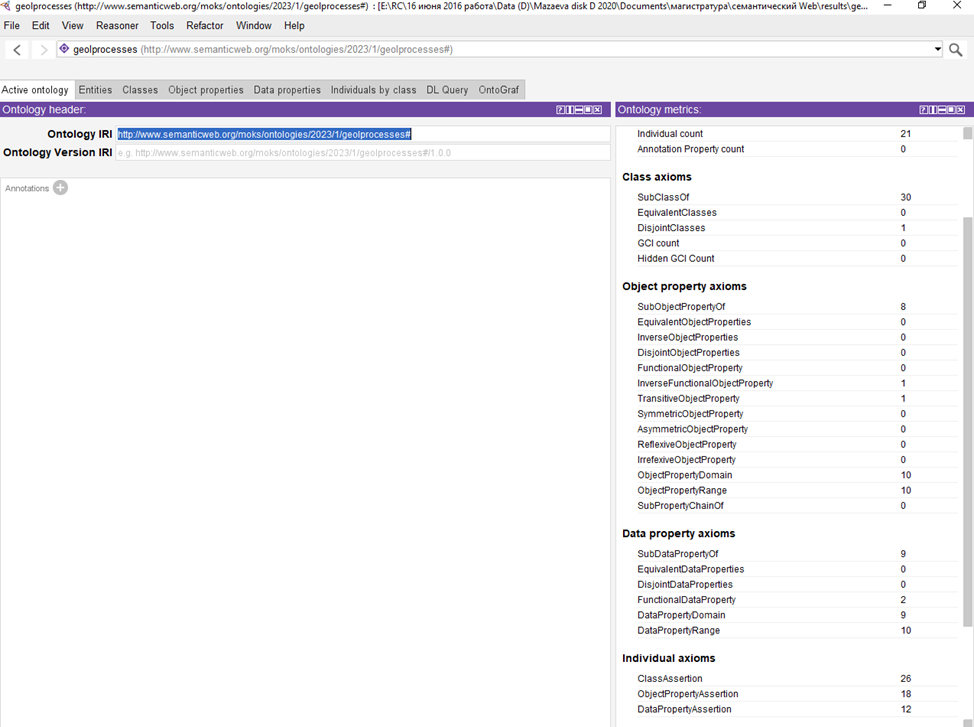
\includegraphics[width=0.9\linewidth]{pics/image19.png}
    \caption{Скриншот экрана панели Ontology metrics с указанием характеристик свойств}
    \label{fig:onto-metrics}
  \end{figure}

  \begin{figure}[htp]
	\centering
	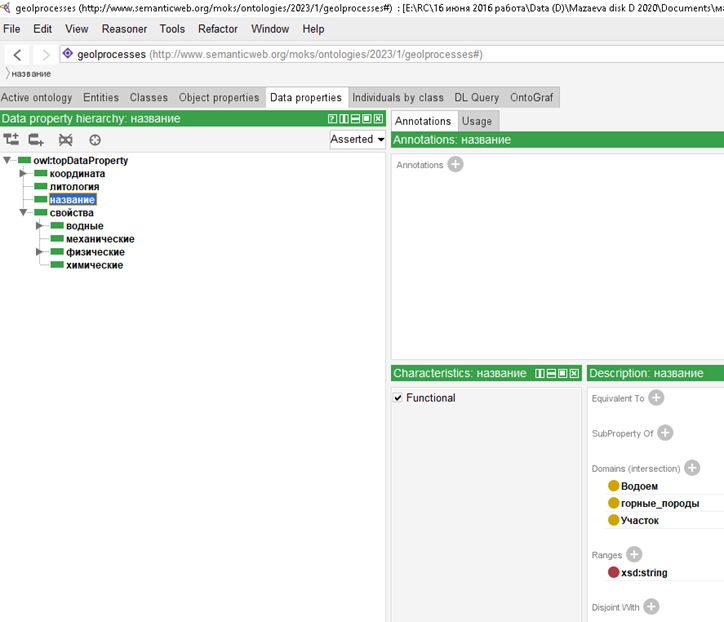
\includegraphics[width=0.9\linewidth]{pics/image8.png}
    \caption{Скриншот экрана панели “Data property” с примером функционального свойства «название»}
    \label{fig:data-props-name}
  \end{figure}

  \begin{figure}[htp]
	\centering
	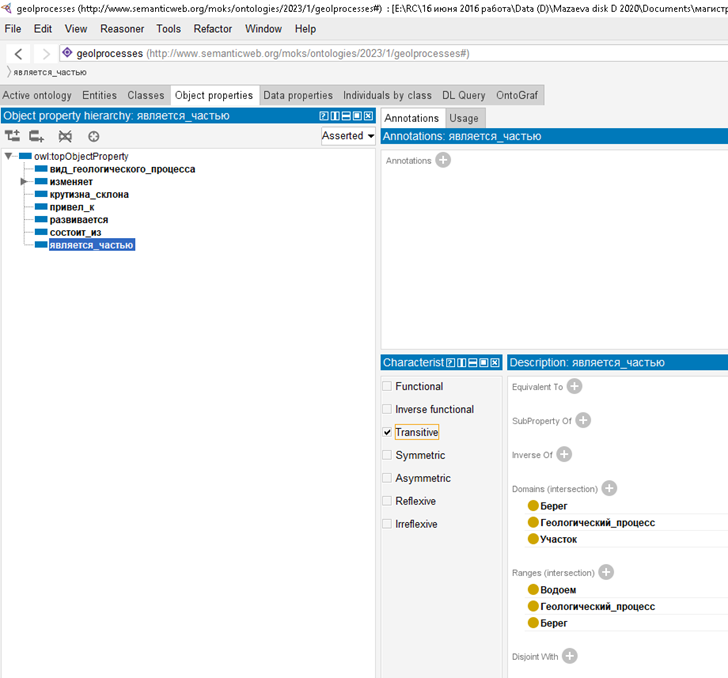
\includegraphics[width=0.9\linewidth]{pics/image11.png}
    \caption{Скриншот экрана панели “Object property” с примером транзитивного свойства «является частью»}
    \label{fig:obj-props-trans}
  \end{figure}

  \begin{figure}[htp]
	\centering
	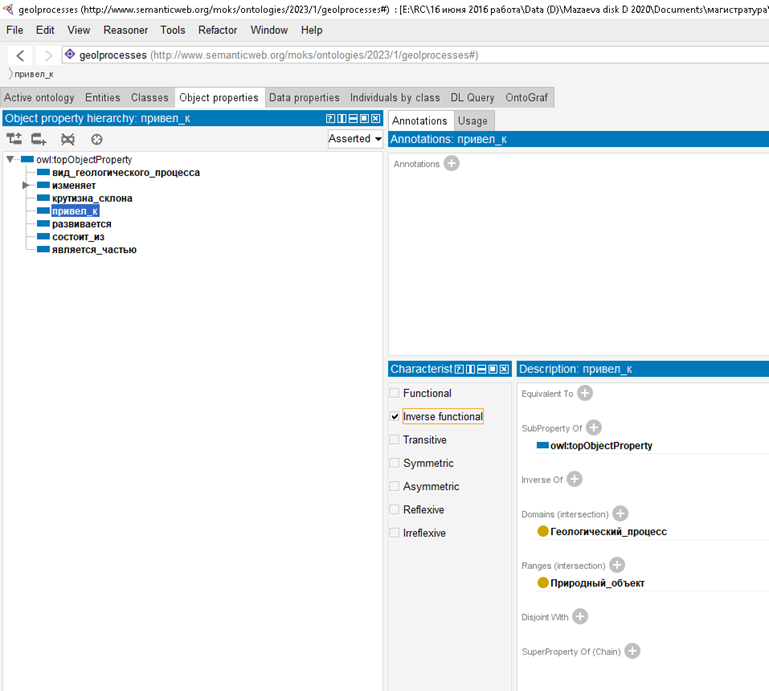
\includegraphics[width=0.9\linewidth]{pics/image7.png}
    \caption{Скриншот экрана панели “Object property” с примером обратно функционального свойства «привел к»}
    \label{fig:obj-prop-results}
  \end{figure}

  \begin{figure}[htp]
	\centering
	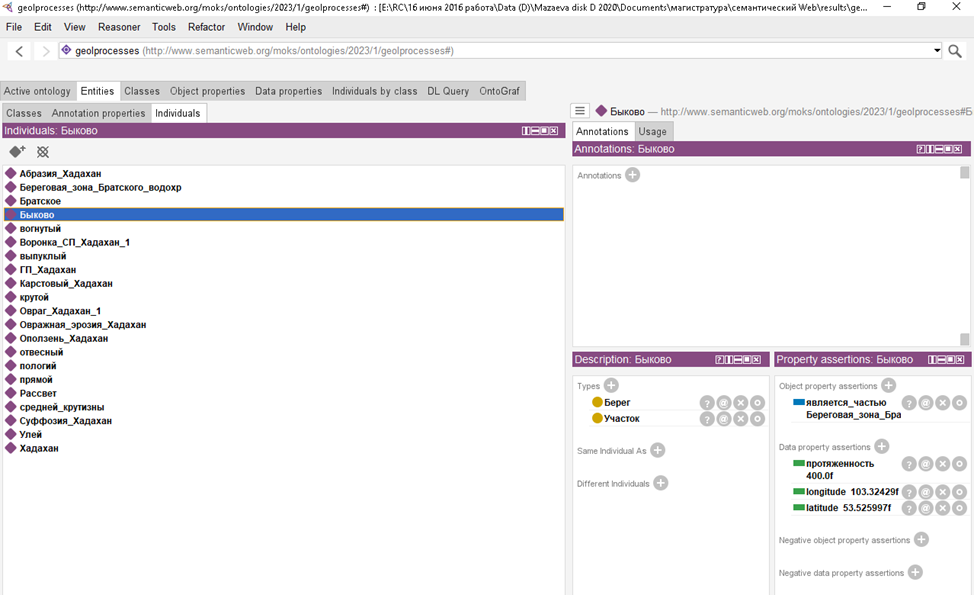
\includegraphics[width=0.9\linewidth]{pics/image5.png}
    \caption{Скриншот экрана с вкладкой “Individuals” для всей онтологии с описанием data property для individuals «Быково»}
    \label{fig:bykovo-instance}
  \end{figure}

Из существующих онтологий в близкой предметной области была найдена онтология UMBEL~\cite{umbel}, описывающая Natural Phenomena (рисунок~\ref{fig:umbel}). В этой онтологии они относятся к SuperType и им дано определение: NaturalPhenomena skos:definition <<Этот SuperType включает в себя природные явления и естественные процессы, такие как погода, выветривание, эрозия, пожары, молнии, землетрясения, тектоника и т.д. Облака и погодные процессы включены особо. Также сюда входят климатические циклы, общие природные явления (например, ураганы), которые не имеют конкретных названий, и биохимические процессы и траектории.>>

  \begin{figure}[htp]
	\centering
	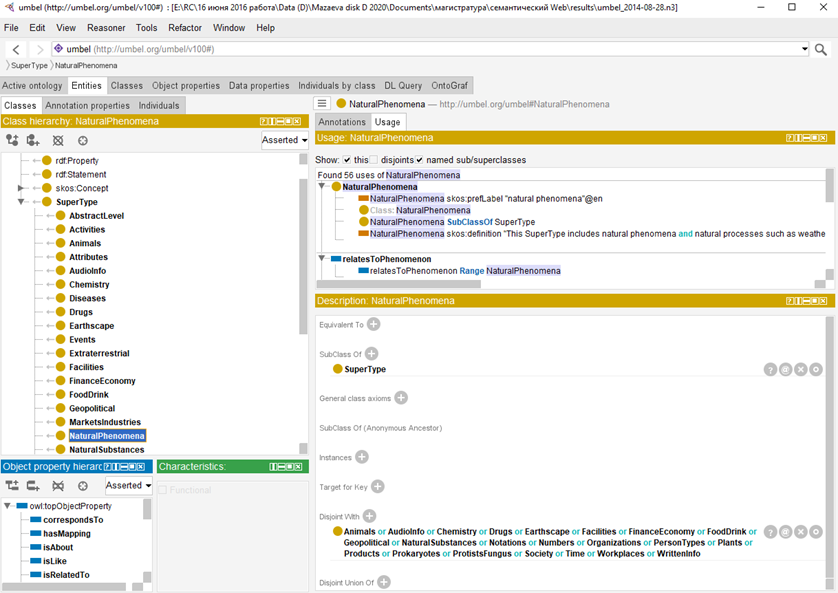
\includegraphics[width=0.9\linewidth]{pics/image14.png}
    \caption{Скриншот экрана существующей онтологии URI http://umbel.org/umbel, описывающая Natural Phenomena}
    \label{fig:umbel}
  \end{figure}

Созданная онтология «Экзогенные процессы на берегах водохранилищ» может быть расширена добавлением водохранилищ, участков, форм экзогенных процессов на участках. Углублена добавлением информации по геологическим и геоморфологическим условиям развития процессов. При добавлении GPS-привязки может использоваться как геоинформационная справочная система для заинтересованных лиц и организаций, а также как база данных для ведения мониторинговых (повторных) наблюдений за экзогенными процессами на берегах водохранилищ.

Данную разработку онтологии можно отнести к комбинированной. Ее создание началось с класса «Водоем» к которому относятся подклассы природных водоемов – «Озеро» и искусственно созданных – «Водохранилище». После были созданы классы «Берег» «Участок» «Форма экзогенного процесса». Все они были объединены в класс «Природный объект» (рисунок~\ref{fig:onto-classes}).

\subsection{Этапы моделирования с использованием DSAS}
\label{sec:model-stages}

Процесс получения результатов прогнозирования с использванием DSAS~\cite{isha20} состоит из следующих этапов:
\begin{enumerate}
\item Оцифровка исходного материала,
\item Представление контуров линий в Shape-файле специального формата,
\item Задание опорной кривой.
\item Передача данных в DSAS (ArcGIS), настройка модуля (шаг трансектов и т.п.).
\item Анализ результатов построения аппроксимации/интерполяции.
\end{enumerate}
Подробно процесс представлен в разделе~\ref{sec:ivi} и русунке~\ref{fig:processes}.

Самой трудоемкой задачей является оконтуривание береговой линии. Как правило, оно делается вручную по снимку (аэро-, спутниковому или ортофотоплан), привязанному к системе координат. Ручное оконтуривание делается при помощи манипулятора “мышь” или графического планшета, в результате получается векторный слой, Shape-файл, контур из которого, потом переносится в набор исходных контуров для DSAS.

В проекте предложено автоматизировать эту операцию при помощи использования современных средств обработки изображений на основе распознавания образов, наборов точек, относящихся к одному объекту. Теперь для получения набора контуров для одной области интереса пользователь сначала в ГИС QGIS выбирает эту область, запускает модуль \verb|shore_qgis_module|, указывает предварительно созданную в проекте пустую группу. В модуле указывается интервал лет, за которые следует проводить распознавания контура, масштаб снимков спутника, адрес спутниковых данных.

Далее модуль запрашивает снимки из хранилищ спутниковых данных, загружает изображения (JPG) на сервер через специальный интерфейс (REST), передающий двоичные данные, принятое сервером изображение раскодируется при помощи библиотеки OpenCV. Изображения сохраняются в виде набора матриц пикселей (RGB) в группе HDF5, соответствующей имени изображения и дате. После сохранения изображения клиент сервера (QGIS-модуль \verb|shore_qgis_module|) запускает процедуру распознавания и периодически опрашивает процессы на сервере на факт их окончания.

Процесс распознавания (SegAny), реализованный на основе Segment Anything, достаточно длительный и требующий достаточно большого объема памяти и вычислительных ресурсов. Результат распознавания помещается в подгруппу группы, хранящей изображение. Результат распознавания представляется как набор масок, обозначающих распознанные объекты, охарактеризованных атрибутами. 

\emph{Маска} - это матрица элементов 0 и 1, где 1 обозначает принадлежность пикселя к распознанному объекту, 0 - нет. Маски не содержат семантической информации, т.е. в данных не указано, что за объект был распознан. Атрибуты масок описывают координату ключевой точки объекта, опоясывающий прямоугольник, площадь маски в пикселях и др.

Для определения контура береговой линии необходимо из набора масок построить две граничащих друг с другом области, где границей выступает береговая линия. Для этого надо определить, какие распознанные объекты являются изображениями области, занятой водой и побережьем (ShRec). Семантику объекта можно определить при помощи запроса к данным OpenstreetMap~\cite{osm}. Для этого делается запрос - “какой объект находится по этой координате”. Если пришел пустой ответ, то запрашивается “Какой объект является наиболее близкий к этой точке”. В запросе указывается тип объекта - элемент рельефа. Все маски, принадлежащие побережью и прибрежной зоне объединяются в одну.

На последнем этапе распознавания нужно построить контур. Для этого используется разработанный в~\cite{b3} алгоритм, преобразующий набор пикселей в векторные данные. Результат записывается в Shape-файл, расположенный в группе, указанной пользователем на начальном этапе. Процедура распознавания SegmentAnything вносит неопределенность в геометрические параметры контура, поэтому пользователь должен проконтролировать результат визуально.

Полученный файл вручную переносится в ArcGIS для применения к ним процедуры DSAS, получение прогноза и интерпретации результатов.

\section{Проектирование информационно-вычислительной инфраструктуры}

Проектирование распределенной вычислительной инфраструктуры является трудоемким процессом, где по мимо реализации алгоритмов конкретных компонент, решаются также вопросы передачи данных между модулями, синхранизация их совместного функционирования. В вкр за время производственной практики разработаны нексколько модулей ИВИ, организован процесс их синхранизации с встроенным в QGIS модулем управления.

\subsection{Функциональные требования}

Совместное использование ГИС и ИВИ предполагает многопользовательскую среду, где разные ГИС делают запросы к сервисам ИВИ на выполнение некоторых задач, требующих больших вычислительны ресурсов, или специальных сервисов. Это включает также обеспечение доступа к данным из разных ГИС (QGIS, ArcGIS и др.). Современные ГИС позволяют обеспечивать доступ пространственно-распределенным данным, представленным в специальных форматах, данным баз реляционных данных, а также виртуальных географических сервисов.

\subsection{Вычислительные процессы в ИВИ}\label{sec:ivi}

В спроектированном распределенном программном комплексе реализуются следующие основные процессы:
\begin{enumerate}
  \item Накопление исходных данных о береговой зоне водохранилища из следующих источников:
  \begin{description}
    \item [Векторные данные ГИС,] получаемые в результате ручной оцифровки или загрузки из топоосновы, привязанные к координатам, \label{lst:target}
    \item [Полевые исследования] в виде координат точек ($x$, $y$, $z$) относительно реперной точки с известными координатами широты и долготы;
    \item [Спутниковые снимки,] получаемые из различных интернет-источников, представленные в форматах JPG, TIFF, JP2 и т.п.;
    \item [Архивные аэрофотоснимки,] требующие сканирования, предварительной обработки проекции, привязки к координатам;
    \item [Ортофотоплан,] формируемый сканированием местности при помощи квадрокоптера, сшивания отдельных снимков, коррекции проекции;
  \end{description}
  \item Оцифровка исходных данных с целью получения данных типа~\ref{lst:target};
  \begin{description}
    \item[Ручная оцифровка] -- исследователь сам анализирует снимок и формирует векторные данные при помощи инструментов ГИС;
    \item[Автоматизированная оцифровка] -- некоторые ГИС позволяют <<обводить>> контуры объектов, ориентируясь на начальную точку контура, указанную человеком, и анализируя разницу цветовых характеристик контура;
    \item[Автоматическая оцифровка,] позволяющая в автоматическом режиме находить на изображении контуры береговой линии (без значитьельного участия человека);
  \end{description}
  \item Подготовка входных данных для построения моделей измерения контура и других характеристик береговой линии;
  \item Вычисление прогноза, и его представление в виде данных ГИС;
  \item Визуализация результатов моделирования и мониторинга;
  \item Интерпретация результатов:
  \begin{description}
    \item[Неавтоматический анализ,] где результаты моделирования анализируются специалистом <<вручную>> и вырабатываются рекомендации по безопасному использованию береговой зоны;
    \item[Автоматизированный анализ,] где часть анализа результата передана экспертной системе.
  \end{description}
\end{enumerate}
На рисунке~\ref{fig:processes} изображены основные описанные выше процессы.

  \begin{figure}[htp]
    \centering
    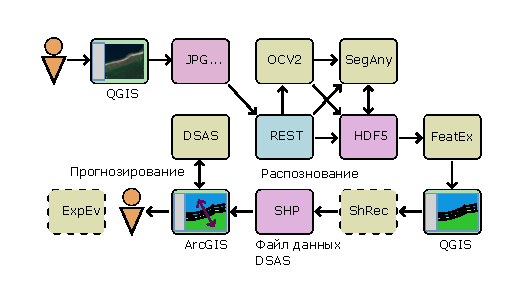
\includegraphics[width=\linewidth]{pics/tech.pdf}
    \caption{Основные процессы в ИВИ поддержки исследований береговых зон водохранилищ}\label{fig:processes}
  \end{figure}

\subsection{Архитектура системы}
Перечисленные в предыдущем разделе функции и взаимодействия между ними формируют собой элементы архитектуры распределенной системы обработки ГИС-данных (рисунок~\ref{fig:arch}).

\begin{figure}[htp]
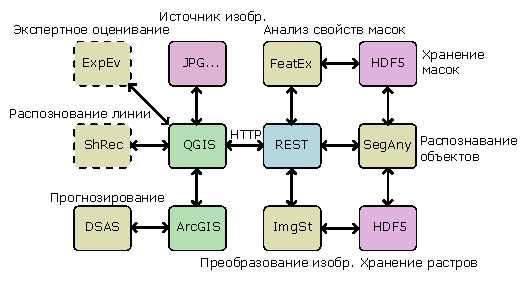
\includegraphics[width=\linewidth]{pics/arch-p.pdf}
  \caption{Архитектура распределенной системы} \label{fig:arch}
\end{figure}

Система состоит из двух основных частей, обычно обозначаемых как <<клиент>> и <<сервер>>. В нашем случае они взаимодействуют друг с другом по протоколу HTTP и реализуют взаимодействие через интерфейс <<архитектуры REST>> (Representation State Protocol). QGIS и ArcGIS - это клиентская часть, она включает также процедуры DSAS, ShRec (распознавание контура), ExpEv (экспертная оценка). QGIS также выступает клиентом для сервера изображений (формат JPG, TIFF, JP2 и др.), получаемых, в том числе, с сервера Google Maps.

Серверная часть -- набор модулей, запускаемых удаленно из модуля \verb|shore_qgis_module|, т.е. процедурами распознавания управляет полностью   клиентская часть. Управление осуществляется через интерфейс REST, где в качестве объектов выступают сервисы хранения исходных изображений (OCV2 + HDF5), распознавания объектов на изображении (SegAny), анализ масок и изображений с целью получения дополнительных характеристик (FeatEx), сервис выгрузки данных с представлением в JSON (внутри REST).

\subsection{Распознавание контура береговой линии}

Как было сказано в разделе, посвященном перечню требований к ИВИ, задача распознавания контура береговой линии решается в условиях ограниченных вычислительных ресурсов и отсутствия предварительно обработанной информации, пригодной для использования современными алгоритмами машинного обучения. Не смотря на данную ситуацию есть возможность применения в задачах распознавания предобученных моделей машинного обучения. 

\subsubsection{Библиотека Segment Anything}
\label{sec:sam}

\emph{SAM (Segment Anything Model)} — это сегментационная модель, которая была выпущена Meta AI*  весной 2023 года и быстро стала одной из самых популярных AI-моделей. SAM называют первой фундаментальной моделью в компьютерном зрении и сравнивают с ChatGPT в NLP из-за рекордно большого количества разнообразных данных, которые видела модель; а также из-за её способности к zero-shot transfer, то есть способности легко обобщаться для решения смежных задач.

SAM обучается на наборе данных Segment Anything 1-Billion mask (SA-1B), который содержит набор из 11 миллионов изображений и более 1 миллиарда масок. Это делает модель очень надежной при определении границ объектов и различении различных объектов в разных доменах, даже если модель никогда раньше с такими объектами не сталкивалась~\cite{samart}.

SAM сегментирует объекты на картинке в соответствии с промптом: им может быть точка на изображении, приблизительный прямоугольник или произвольный текст. Авторы отмечают, что при заранее вычисленном эмбеддинге изображения модель способна работать на CPU в браузере в реальном времени, а также может применяться без дообучения для задач, отличных от сегментации (например, для задач детекции границ и положения объектов — edge detection и object proposal).

Кодер изображений реализован в PyTorch, и для эффективного вывода требуется графический процессор. Кодер подсказок и декодер маски могут работать непосредственно с PyTroch или конвертироваться в ONNX и эффективно работать на ЦП или графическом процессоре на различных платформах, поддерживающих среду выполнения ONNX~\cite{samart}.

\subsection{Анализ структуры объектов изображения}

На данном этапе производится классификация объектов -- необходимо соотнести распознанные объекты к классам <<водная поверхность>> и <<суша>>. Модель SA для каждого распознанного объекта сопоставляет так называемую ключевую точку (рисунок~\ref{fig:objsanalysis}). В режиме распознавания <<всех объектов>> на изображении библиотека сканирует изображения по некоторой сетке. Каждой точкой сетки производится указание (prompt) на объект, который необходимо выделить на изображении. Если указанию соответствует новый объект, то этот объект ассоциируется с точкой. Получается, что координаты ключевой точки идентифицируют объект.

\begin{figure}
  \centering
  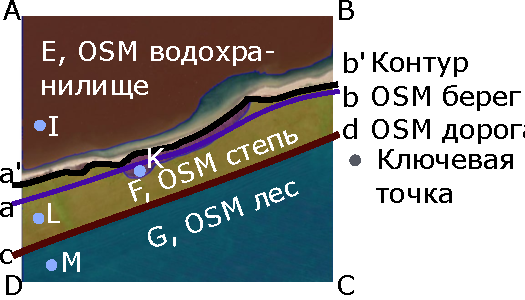
\includegraphics[width=0.7\linewidth]{pics/tracing-p.pdf}
  \caption{К объяснению идеи распознавания береговой линии при помощи классификации масок SsegmentAnything}\label{fig:objsanalysis}
\end{figure}

На рисунке~\ref{fig:objsanalysis} точки A, B, C, D обозначают периметр изображения, координаты которого используется для определения свойств объектов (например, как касающихся границы), объекты E, F, G -- собственно некоторые распознанные объекты. Кружочками обозначены ключевые точки, координаты которых идентифицируют объекты. Таким образом, объекты F, G, и объект, идентифицируемый K -- это берег водохранилища, содержащий нужный контур a’--b’. Кривая a--b -- граница водохранилища, полученная с OpenStreetMap, ее можно использовать как <<начальное приближение>> или опорный объект выделения множества граничных точек объединенного контура берега. Кривая c--d (дорога вдоль границы леса) принадлежит побережью и находится дальше от ab, чем a’--b’ и не может быть побережьем. Дополнительные свойства объектов, используемые для фильтрации получаются запуском процедуры совместного анализа данных масок (FeatEx) и изображения с целью порождения дополнительных атрибутов объектов, например, средний цвет объекта, расстояние границы объекта к границе изображения, общая граница с другими объектами и т.п.

Точка, таким образом, принадлежит объекту, точнее находится на маске изображения. Чтобы достаточно достоверно определить, является объект водным или сушей, можно выполнить запрос к серверу OpenStreetMap~\cite{osm} следующего вида:
\begin{minted}{text}
  [out:json];
    (
      is_in(53.5202071,103.3259833); // Координата точки K
    );
    out center;
\end{minted}
В ответ будет получен JSON следующего вида:
\begin{minted}{json}
  {
  "version": 0.6,
  "generator": "Overpass API 0.7.62.1 084b4234",
  "osm3s": {
    "timestamp_osm_base": "2024-06-12T10:11:58Z",
    "timestamp_areas_base": "2024-06-12T05:25:19Z",
    "copyright": "The data included in this document is from www.openstreetmap.org. The data is made available under ODbL."
  },
  "elements": [

{
  "type": "area",
  "id": 3600060189,
  "tags": {
    "ISO3166-1": "RU",
    "ISO3166-1:alpha2": "RU",
    "ISO3166-1:alpha3": "RUS",
    "ISO3166-1:numeric": "643",
    "according_to:RU": "yes",
    "according_to:UA": "no",
    "admin_level": "2",
    "alt_name:eo": "Rusujo;Ruslando",
    "border_type": "nation",
    "boundary": "administrative",
    "currency": "RUB",
    "default_language": "ru",
    "flag": "https://upload.wikimedia.org/wikipedia/commons/f/f3/Flag_of_Russia.svg",
    "int_name": "Russia",
    "int_ref": "RU",
    "name": "Россия",
  // .....
},
// ....
{
  "type": "area",
  "id": 3601221148,
  "tags": {
    "addr:country": "RU",
    "admin_level": "3",
    "boundary": "administrative",
    // .....
}
// ....
\end{minted}
Среди перечисленных объектов нет объекта, обозначающего водный резервуар. Теперь запрос по координате точки $I$:
\begin{minted}{text}
  [out:json];
    (
      is_in(53.5202071,103.3259833); // Координата точки I
    );
    out center;
\end{minted}
В ответ будет получен JSON следующего вида:
\begin{minted}{json}
// ......
{
  "type": "area",
  "id": 3600167043,
  "tags": {
    "alt_name:cs": "Bratská vodní nádrž",
    "gvr:code": "16010100821416200001042",
    "name": "Братское водохранилище",
    "name:ca": "Embassament de Bratsk",
    "name:cs": "Bratská přehradní nádrž",
    "name:en": "Bratsk Reservoir",
    "name:eo": "Bratska Rezervujo",
    "name:pl": "Zbiornik Bracki",
    "name:ru": "Братское водохранилище",
    "name:sk": "Bratská vodná nádrž",
    "name:zh": "布拉茨克水库",
    "natural": "water",
    "type": "multipolygon",
    "water": "reservoir",   // Тег, определяющий тип водема
    "wikidata": "Q899803",
    "wikipedia": "ru:Братское водохранилище"
  }
},
// ......
\end{minted}
Здесь среди выданных объектов присутствует объект, описанный как водный резервуар.

Собрав информацию по всем ключевым точкам, теперь становиться возможным объединить все маски, относящиеся к водным объектам, и все маски, относящиеся к суше. Граница суши со стороны водного объекта будет являться приближением береговой линии. Контур береговой линии $a'$--$b'$ из набора пикселей (растра) преобразуется в векторный объект при помощи варианта алгоритма, представленного в \cite{b3}.

Предлагаемый подход также применим к привязанным к координатам аэрофотоснимкам и ортофотопланам.

\chapter{Реализация подсистем распределенной вычислительной среды}\label{chap:impl}

За время работы над задачей реализации ГИС береговой зоны разработаны некоторые модули подсистемы, изображенные на рисунке~\ref{fig:arch} непрерывными линиями.

\section{Модуль управления процессом моделирования}

Данный модуль реализован в виде расширения QGIS. Модули расширения реализуются согласно стандартизованной технологии включающей
\begin{itemize}
\item интерфейс пользователя, проектируемый при помощи QT-дизайнера,
\item класс, реализующий конкретные функции.
\end{itemize}

Интерфейс пользователя, реализованный в модуле изображен на рисунке~\ref{fig:plugin-ui}. Управление модулем производится при помощи панели в трее. Интерфейс включает четыре вкладки: выбор целевой группы слоев, в которую будет помещаться результат распознавания в виде shape-файла; Выбор тайл-слоя, откуда загружается изображение для анализа; перечень сгенерированных shape-слоев; настройка модуля, в частности, адрес сервера хранения и обработки изображений.
  \begin{figure}[htp]
    \centering
    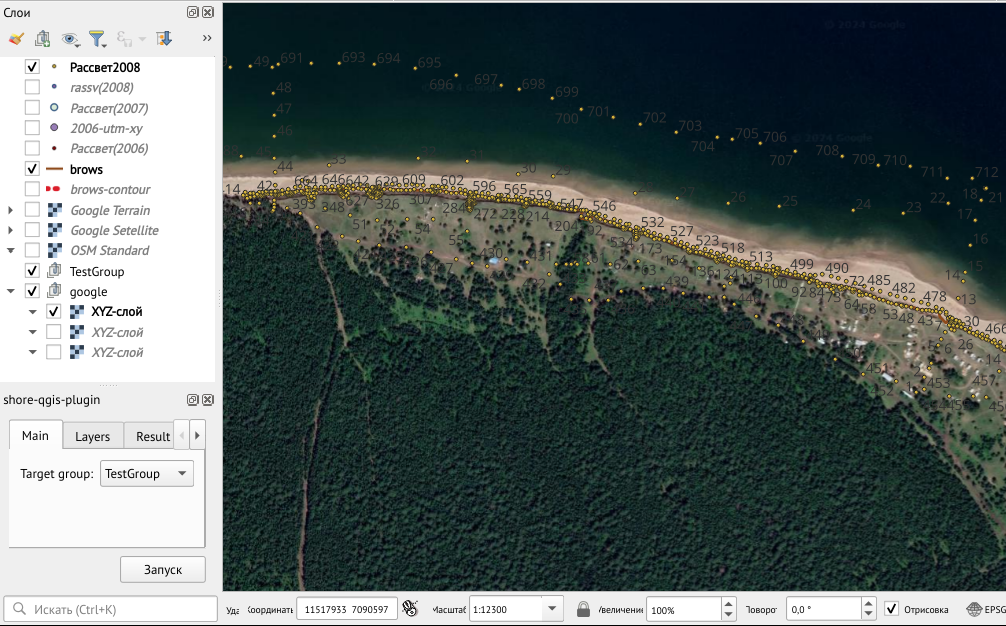
\includegraphics[width=\linewidth]{pics/plugin-ui.png}
    \caption{Интерфейс пользователя, реализованный в модуле расширения}
    \label{fig:plugin-ui}
  \end{figure}

Задача модуля -- координировать процесс обработки изображений. Взаимодействие модуля с сервером осуществляется через интерфейс (модуль) REST.

\section{Интерфейс REST загрузки и обработки изображений}

REST (Representational state transfer) – это стиль архитектуры программного обеспечения для распределенных систем, таких как World Wide Web, который, как правило, используется для построения веб-служб. Термин REST был введен в 2000 году Роем Филдингом, одним из авторов HTTP-протокола. Системы, поддерживающие REST, называются RESTful-системами.

В общем случае REST является очень простым интерфейсом управления информацией без использования каких-то дополнительных внутренних прослоек. Каждая единица информации однозначно определяется глобальным идентификатором, таким как URL. Каждая URL в свою очередь имеет строго заданный формат.

Задача интерфейса REST - принимать бинарный файл изображения, преобразовать его в матрицы слоев, записать в базу данных на сервере, выдать глобальный идентификатор, при помощи которого далее идентифицируется сохраненные данные изображения, запуск других подсистем. Приведем пример реализации интерфейсов REST для загрузки изображений и управления процессом распознавания.

\begin{minted}{python}
img = Service(name='imgstore',
              path='/sa-1.0/image/{img_name}',
              description="Image collection")

@img.put()
def put_image(request):
    """Принимает бинарные данные картинки,
    возвращает JSON с UUID сохраненного изображения
    """
    name = request.matchdict['img_name']

    imgg, ds = add_image(name, request.body)

    uui = uuidgen()
    uuis = str(uui)
    pth = ds.name
    STORAGE, INGRP, UUIDGRP = storage_begin()
    if name in UUIDGRP:
        ouuis = gs(UUIDGRP[name])
        del UUIDGRP[name]
        del UUIDGRP[ouuis]
    # Отображение UUID <-> имя изображения
    UUIDGRP.create_dataset(name, data=uuis)
    UUIDGRP.create_dataset(uuis, data=name)
    STORAGE, INGRP, UUIDGRP = storage_end()
    return {
        "error": None,
        "ok": True,
        "uuid": uuis,
        "content": pth,
        "name": name,
        "namepath": imgg.name
    }

def add_image(name, content, replace=True):
    ”””Добавление изображения в БД”””
    nparr = np.frombuffer(content, np.uint8)
    image = cv2.imdecode(nparr, cv2.IMREAD_COLOR)
    image = cv2.cvtColor(image, cv2.COLOR_BGR2RGB)
    # Открытие БД
    STORAGE, INGRP, UUIDGRP = storage_begin()
    if name in INGRP:
        del INGRP[name]
    imgg = INGRP.create_group(name)
    ds = imgg.create_dataset('content',
              data=image, compression="lzf")
    log.info("Image '{}' loaded".format(name))
    # Закрытие БД
    STORAGE, INGRP, UUIDGRP = storage_end()
    return (imgg, ds)
\end{minted}

Загрузка изображения делается при помощи запроса PUT с адресом \verb|https://<адрес сервера>:6543/sa-1.0/image/<имя картинки>|. В тело запроса PUT помещается содержимое изображения. В качестве результата возвращается JSON-ответ, содержащий в поле <<uuid>> идентификатор сохраненного изображения. Список сохраненных изображений получается запуском запроса GET к этому же адресу без указания имени изображения. Возвращается JSON со списком отображений UUID-<имя файла изображения>. Полученный идентификатор используется для обозначения изображения, подвергающегося процедуре распознавания:

\begin{minted}{python}
sactrl = Service(name='segment-any-control',
                 path='/sa-1.0/sa/{img_uuid}/{cmd}',
                 description="Functions of SA on a image\
                              identified by uuid")
@sactrl.post()
def start_recognition(request):
    # Импорт процедур анализа, выполняющихся в
    #  других процессах
    from ..tasks import (sa_start,
          ANSWERS, rc_set, rc_get, rc_delete,
          rc_update)

    uuids = request.matchdict['img_uuid']
    cmd = request.matchdict['cmd']
    # cmd = 'start'

    STORAGE, INGRP, UUIDGRP = storage_begin()
    # идентификатор изображения существует?
    isimg = uuids in UUIDGRP
    STORAGE, INGRP, UUIDGRP = storage_end()

    rd = {"error": False, "ok": True, "cmd": cmd}

    if cmd == "flush":
        ANSWERS.flushdb()
        return rd

    if not isimg:
        return {
            "error": "not found",
            "ok": False,
            "uuid": uuids,
            "cmd": cmd,
            "processuuid": None
        }
    # Команда запуска процесса распознавания
    if cmd == "start":
        prevrc = rc_get(uuids)
        if prevrc is not None:
            return {
                "error": "already running",
                "ok": False,
                "uuid": uuids,
                "cmd": cmd,
                "processuuid": prevrc.get("processuuid",
                                           None),
                "ready": prevrc.get("ready", False)
            }
        del prevrc
        rc = {"uuid": uuids, "ready": False}
        rc_set(uuids, rc)
        arc = sa_start.delay(uuids)
        puuid = str(arc.id)

        def _u(r):
            r["processuuid"] = puuid

        rc = rc_update(uuids, _u)
        print(rc_get(uuids))
        puuid = rd["processuuid"] = puuid
    # Команда проверки завершения процесса
    elif cmd == "status":
        rd["ready"] = False

        def _a(v, rr):
            rd["ready"] = v
            rd["result"] = rr.get("result", None)

        rc = rc_get(uuids, "ready", _a)
        if rc is None:
            return {
                "error": "no process",
                "ok": False,
                "uuid": uuids,
                "cmd": cmd,
                "ready": None
            }

        rd["processuuid"] = rc["processuuid"]
    # Команда завершения процесса и удаления его данных
    elif cmd == "finalize":
        rcg = rc_get(uuids)
        if rcg is None:
            return {
                "error": "not running",
                "ok": False,
                "uuid": uuids,
                "cmd": cmd,
                "ready": None
            }
        rc_delete(uuids)
        rd.update({"ready": rcg["ready"],
                   "processuuid": rcg["processuuid"]})
    # Команда отмены процесса
    elif cmd == "discard":
        rcg = rc_get(uuids)
        if rcg is not None:
            return {
                "error": "still running",
                "description":
                "cannot stop SA, wait its finishing. \
                     Use status command.",
                "ok": False,
                "uuid": uuids,
                "cmd": cmd,
                "ready": None
            }
        STORAGE, INGRP, UUIDGRP = storage_begin()
        name = gs(UUIDGRP[uuids])
        imgg = INGRP[name]
        if "masks" in imgg:
            del imgg["masks"]
            rc = "removed"
        else:
            rc = "no mask"
        STORAGE, INGRP, UUIDGRP = storage_end()
        rd.update({
            "ready": None,
            "processuuid": None,
            "description": rc
        })

    return rd
\end{minted}

Запуск процесса распознавания осуществляется при помощи запроса POST следующего формата - \texttt{http://<адрес сервера>:6543/sa-1.0/sa/<идентификатор изображения>/<команда>}. Командой выступает ключевое слово - одно из четырех:
\begin{description}
  \item[start] -- запуск нового процесса,
  \item[status] -- запрос состояния распознавания,
  \item[finalize] -- завершение исполнившегося процесса,
  \item[flush] -- отмена процесса.
\end{description}
Требующие большие вычислительные ресурсы процессы выполняются в отдельных процессах сервера или на специализированных серверах, снабженных аппаратной поддержкой вычислений (CUDA и ему подобным). Реализация запуска таких задач реализована при помощи библиотеки celery языка программирования Python.

\section{Исполнение задач с долгим времением вычисления}

На этапе предварительного ознакомления с библиотекой SegmentAnything было установлено, что среднее время выполнения распознавания объектов на изображении, взятом с Google-сервера - 3.5 минуты на персоналном компьютере, оборудованом ОС Linux, видеокартой NVIDIA 1030 и использование библиотеки \verb|tensorflow| с поддержкой CUDA. Если операцию напосредственно выполнять из интерфейса пользователя, то работа с ГИС QGIS для пользователя будет некомфортной -- он должен будет ждать результата, но при этом не будет возможности выполнять какие-либо другие операции. Для решения этой проблемы и бвл разработан сервер хранения и обработки изображений. Пользователи задают задачи <<длительного выполнения>>, задачи ставятся в очередь на сервере, по завершению их исполнения модуль QGIS запрашивает результат и помещает его в проект.

Реализация очереди выполнена при помощи отдельного объекта REST и процесса - сервера очередей \verb|celery| (сельдерей). Работа очереди обеспечивается еще одним дополнительным сервисом -- \verb|RabbitMQ| -- <<Rabbit>> message queue, ранее установленным в сети ИДСТУ как раз для поддержки очередей. RabbitMQ позволяет синхронизировать вычислительные процессы на основе организации передачи сообщений, а также распределять нагрузку между вычислительными узлами, что дает возможность разрабатыват масштабируемые ИВИ. 

\section{Хранение изображений}

Загруженное через REST-интерфейс изображение декодируется и преобразуется в набор матриц (тензор), соответствующий слоям Red-Green-Blue-Alpha. Преобразование осуществляется перед выполнением сохранения. Такой подход позволяет на этапе передачи изображения на обработку загружать данные непосредственно из хранилища в модули обработки в виде объектов numpy. Идея реализована при помощи файлов формата HDF5.

\subsection{Стандарт HDF5: формат и инструментарий}

Иерархический формат данных версии 5 (HDF5) - это формат файлов с открытым исходным кодом, который поддерживает большие, сложные и неоднородные данные. HDF5 использует структуру типа "файловый каталог", которая позволяет организовывать данные внутри файла множеством способов, как это делается в папках на вашем компьютере. Формат HDF5 также позволяет встраивать метаданные, делая его самоопределяющимся.

HDF5 — современная версия формата. Получил премию R\&D100 от журнала <<R\&D Magazine>> в 2002 году~\cite{hdf5}.
Содержит иерархию из двух основных типов объектов:
\begin{description}
\item [Datasets] — наборы данных, многомерные массивы объектов одного типа
\item [Groups] — группы, являются контейнерами для наборов данных и других групп
\end{description}

Содержимое файлов HDF5 организовано подобно иерархической файловой системе, и для доступа к данным применяются пути, сходные с POSIX-синтаксисом, например, /path/to/resource. Метаданные хранятся в виде набора именованных атрибутов объектов (рисунок~\ref{fig:hdf5-example}.
  \begin{figure}[htp]
    \centering
    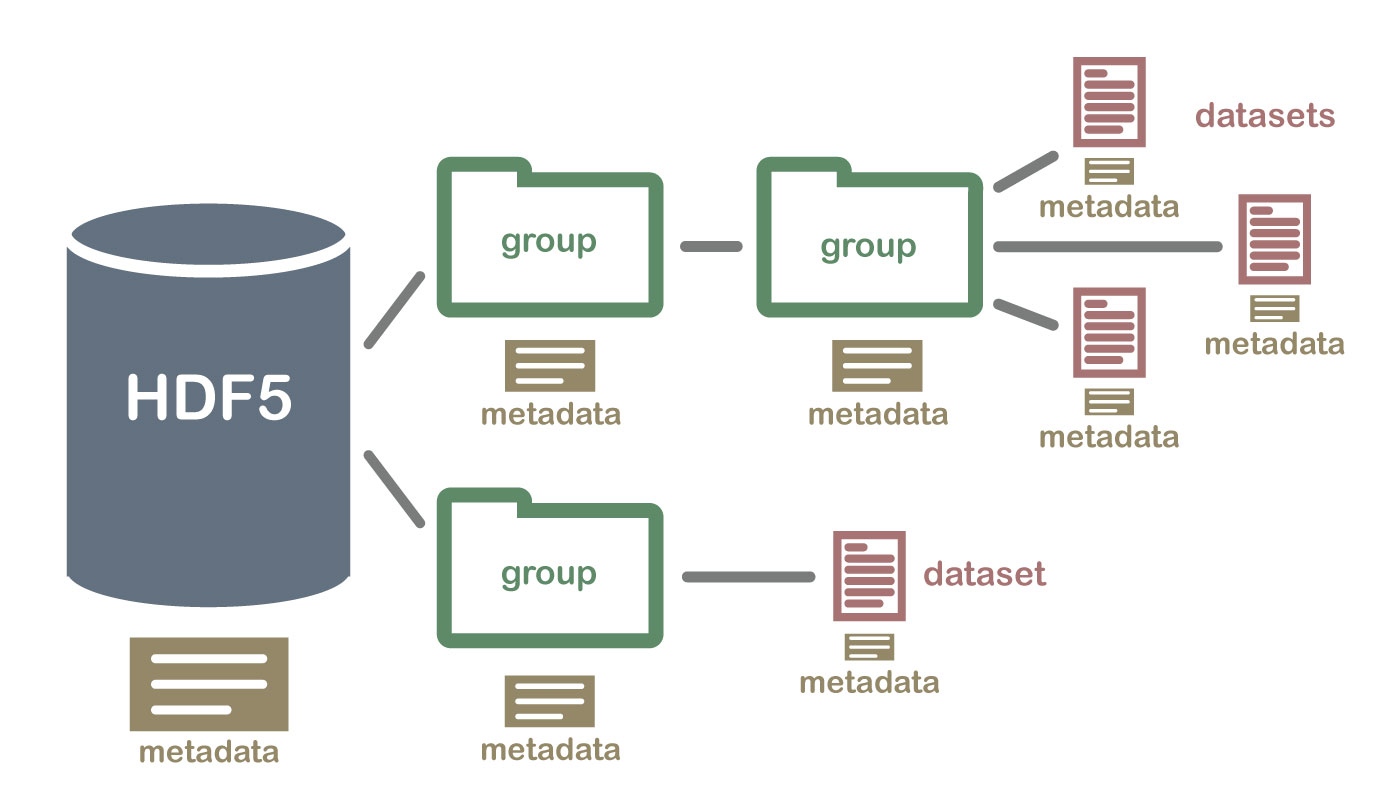
\includegraphics[width=0.7\linewidth]{pics/hdf5_structure4.jpg}
    \caption{Вариант хранения информации в формате HDF5}
    \label{fig:hfd5-example}
  \end{figure}

\subsection{Хранение изображений и масок}

Изображения, преобразованные в тензоры, сохраняются в корневой узел хранения изображений в виде группы, поименованной именем файла изображения. Маски, распознанные на изображении помещаются в подруппу <<masks>>. Тензор изображения помещается в узел <<content>>. Сгенерированный идентификатор (UUID) помещается в атрибут группы изображения, а также в специальный узел отображения идентификаторов в имена изображений и обратно. Тензоры изображений сжимаются алгоритмом LZW, использование которого позволяет загружать тензор прямым проходом по данным. Маски также содержат узел <<content>>, к которому привязаны атрибуты, ассоциированными с маской.

Доступ к данным изображения, масок, атрибутам и т.п. реализован также в интерфейсе REST. В частности, маски выгружаются по порядковым номерам и идентификаторам соответствующего изображения.

\section{Тестирование}

К текущему моменту реализованы не все модули представленной в ВКР архитектуры, поэтому подемонстрируем только работоспособное взаимодействие пользователя, модуля QGIS, сервера обработки изображений. Вычислительный процесс начинается с момента нажатия кнопки <<Запуск>> в интерфейсе модуля QGIS. До этого, как было сказано выше, пользователь должен создать проект, подключить XYZ Tile Layer, например, Google Maps, поставляющий растровые данные спутниковых изобраений. Также необходимо установить интересующий регион при помощи манипуляции с картами и визуальным контролем.

Модуль получает изображения Tile-слоя в виде JPG-изображения и посылвет его на сервер при помощи запроса PUT (для наглядности мы моделируем запрос при помощи программы curl):
\begin{minted}{text}
$ curl -X PUT http://127.0.0.1:6543/sa-1.0/image/Bykovo.jpg --data-binary "@Bykovo6.JPG"
{"error": null, "ok": true, "uuid": "a535ef20-2b7b-11ef-9f92-704d7b84fd9f", "content": null, "name": "Bykovo.jpg", "namepath": null}
\end{minted}

В результате получен ответ: операция проведена успешно, изображение помещено в хранилище в виде тензора под идентификатором <<a535ef20-2b7b-11ef-9f92-704d7b84fd9f>>. Далее данный идентификатор будетимпользоваться для указания тензора. На запрос сервер отреагировал записью в жкрнале:

\begin{minted}{text}
Starting server in PID 14014.
2024-05-16 08:49:41,197 INFO  [waitress:485][MainThread] Serving on http://127.0.0.1:6543
2024-05-16 08:49:41,198 INFO  [waitress:485][MainThread] Serving on http://[::1]:6543
2024-05-16 08:59:12,365 INFO  [shores_server.views.rest:44][waitress-1] Successfully opened the database
2024-05-16 08:59:12,427 INFO  [shores_server.views.rest:149][waitress-1] Image 'Bykovo.jpg' loaded
2024-05-16 08:59:12,453 INFO  [shores_server.views.rest:44][waitress-1] Successfully opened the database
\end{minted}

Далее запускаем процесс распознавания объектов, передавая идентификатор тензора и указывая команду \verb|start|:
\begin{minted}{text}
$ curl -X POST http://127.0.0.1:6543/sa-1.0/sa/a535ef20-2b7b-11ef-9f92-704d7b84fd9f/start
{"error": false, "ok": true, "cmd": "start", "processuuid": "bc31a029-8cc6-4c9d-803f-7f46d2b10def"}
\end{minted}
Возврашено сообщение о том, что процесс запущен и идентификатор этого процесса.

Журнал REST-модуля дополняется записью
\begin{minted}{text}
2024-05-16 08:59:12,427 INFO  [shores_server.views.rest:149][waitress-1] Image 'Bykovo.jpg' loaded
2024-05-16 08:59:12,453 INFO  [shores_server.views.rest:44][waitress-1] Successfully opened the database
2024-05-16 09:04:18,513 INFO  [shores_server.views.rest:44][waitress-3] Successfully opened the database
{'uuid': 'a535ef20-2b7b-11ef-9f92-704d7b84fd9f', 'ready': False, 'processuuid': 'bc31a029-8cc6-4c9d-803f-7f46d2b10def'}
\end{minted}
  
Сервер clery реагирует на сообщение
\begin{minted}{text}
    -------------- celery@center.irnok.net v5.3.6 (emerald-rush)
--- ***** -----
-- ******* ---- Linux-6.6.30-1-lts-x86_64-with-glibc2.39 2024-06-16 08:49:41
- *** --- * ---
- ** ---------- [config]
- ** ---------- .> app:         __main__:0x7bc3a2b065a0
- ** ---------- .> transport:   amqp://shores:**@192.168.191.131:5672/shores
- ** ---------- .> results:     sqlite:///results.db
- *** --- * --- .> concurrency: 4 (prefork)
-- ******* ---- .> task events: OFF (enable -E to monitor tasks in this worker)
--- ***** -----
  -------------- [queues]
                .> celery           exchange=celery(direct) key=celery


2024-05-16 08:49:43,119 WARNI [py.warnings:110][MainThread] /home/eugeneai/.pyenv/versions/3.12.2/envs/shores-server/lib/2024-05-16 08:49:43,354 INFO  [celery.worker.consumer.connection:22][MainThread] Connected to amqp://shores:**@192.168.191.131:5672/shores
2024-05-16 08:49:43,358 WARNI [py.warnings:110][MainThread] /home/eugeneai/.pyenv/versions/3.12.2/envs/shores-server/lib/python3.12/site-packages/celery/worker/consumer/consumer.py:507: CPendingDeprecationWarning: The broker_connection_retry configuration setting will no longer determine
whether broker connection retries are made during startup in Celery 6.0 and above.
2024-05-16 08:49:43,435 INFO  [celery.worker.consumer.mingle:40][MainThread] mingle: searching for neighbors
2024-05-16 08:49:44,745 INFO  [celery.worker.consumer.mingle:49][MainThread] mingle: all alone
2024-05-16 08:49:45,092 INFO  [celery.apps.worker:175][MainThread] celery@center.irnok.net ready.
...
2024-05-16 09:04:18,804 INFO  [celery.worker.strategy:161][MainThread] Task shores_server.tasks.sa_start[bc31a029-8cc6-4c9d-803f-7f46d2b10def] received
2024-05-16 09:04:18,812 INFO  [shores_server.tasks:187][MainThread] creating task processing image identified by UUID a535ef20-2b7b-11ef-9f92-704d7b84fd9f
2024-05-16 09:04:18,819 INFO  [shores_server.views.rest:44][MainThread] Successfully opened the database
2024-05-16 09:04:18,830 INFO  [root:191][MainThread] Image name is 'Bykovo.jpg'
2024-05-16 09:04:18,896 INFO  [root:195][MainThread] Image shape is (979, 1568, 3)
2024-05-16 09:04:18,897 INFO  [root:203][MainThread] New recognition starting.
2024-05-16 09:04:18,898 INFO  [root:205][MainThread] Torch engine is cpu.
2024-05-16 09:04:18,898 INFO  [root:92][MainThread] SAM starts loading
2024-05-16 09:04:25,912 INFO  [root:102][MainThread] SAM loaded 'vit_b'
2024-05-16 09:04:25,912 INFO  [root:115][MainThread] Start Recognition/Segmentation
2024-05-16 09:06:09,571 INFO  [root:117][MainThread] Finish Recognition/Segmentation
2024-05-16 09:06:09,571 INFO  [root:216][MainThread] Recognition finished, saving into storage.
2024-05-16 09:06:09,573 INFO  [shores_server.views.rest:44][MainThread] Successfully opened the database
2024-05-16 09:06:09,632 INFO  [root:243][MainThread] Found 8 masks
2024-05-16 09:06:09,891 INFO  [celery.app.trace:131][MainThread] Task shores_server.tasks.sa_start[bc31a029-8cc6-4c9d-803f-7f46d2b10def] succeeded in 111.08417257107794s: None
\end{minted}
Сервер SegmentAnything загрузил модель, передал управление процедуре распознавания, SA распознал 8 объектов, эти объекты помещены в HDF5-хранилище в виде масок.

Маски выгружаются с сервера при помощи следующего запроса:
\begin{minted}{text}
$ curl -X GET http://127.0.0.1:6543/sa-1.0/mask/a535ef20-2b7b-11ef-9f92-704d7b84fd9f/0
{"error": false, "ok": true, "result": {"area": 674868, "predicted_iou": 1.0044816732406616, "stability_score": 0.9672640562057495, "bbox": [625, 0, 942, 945], "crop_box": [0, 0, 1568, 979], "point_coords": [[1151.5, 627.171875]], "segmentation": [[0, 0, 0, 0, 0, 
.....
0, 0, 0, 0, 0, 0, 0, 0, 0, 0, 0, 0, 0, 0, 0, 0, 0]]}}
\end{minted}

Сервер реагирует, в его журнал добавляется запись (факт доступа к HDF5-хранилищу):
\begin{minted}{text}
2024-05-16 09:14:29,200 INFO  [shores_server.views.rest:44][waitress-0] Successfully opened the database
2024-05-16 09:14:29,208 INFO  [shores_server.views.rest:44][waitress-0] Successfully opened the database 
\end{minted}

Далее можно запустить еще один процесс, процесс изъятия значений для характеристик масок и представление их в виде графа знаний, но сначала надо сообщить серверу, что мы завершилии работу с модулем SA:
\begin{minted}{text}
$ curl -X POST http://127.0.0.1:6543/sa-1.0/sa/a535ef20-2b7b-11ef-9f92-704d7b84fd9f/finalize
{"error": false, "ok": true, "cmd": "finalize", "ready": true, "processuuid": "bc31a029-8cc6-4c9d-803f-7f46d2b10def"}
# Запуск feature extraction
$ curl -X POST http://127.0.0.1:6543/sa-1.0/fe/a535ef20-2b7b-11ef-9f92-704d7b84fd9f/start
{"error": false, "ok": true, "cmd": "start", "processuuid": "1ee19583-ae48-471f-9081-25b840510d3c"}
# Запрос статуса операции - завершен
$ curl -X POST http://127.0.0.1:6543/sa-1.0/fe/a535ef20-2b7b-11ef-9f92-704d7b84fd9f/status
{"error": false, "ok": true, "cmd": "status", "ready": true, "result": true, "processuuid": "1ee19583-ae48-471f-9081-25b840510d3c"}
# Завершение задачи feature extraction
$ curl -X POST http://127.0.0.1:6543/sa-1.0/fe/a535ef20-2b7b-11ef-9f92-704d7b84fd9f/finzlize
{"error": false, "ok": true, "cmd": "finzlize"}
\end{minted}

Журнал Celery:
\begin{minted}{text}
2024-05-16 09:21:48,141 INFO  [celery.worker.strategy:161][MainThread] Task shores_server.tasks.feature_recognition[1ee19583-ae48-471f-9081-25b840510d3c] received
2024-05-16 09:21:48,144 INFO  [shores_server.tasks:268][MainThread] Creating task processing masks for image identified by UUID a535ef20-2b7b-11ef-9f92-704d7b84fd9f
2024-05-16 09:21:48,144 INFO  [shores_server.views.rest:44][MainThread] Successfully opened the database
2024-05-16 09:21:48,228 INFO  [root:300][MainThread] Starting FE on (979, 1568, 3) shape image and 8 its masks
\end{minted}
В результате формируется граф знаний, приведенный в Приложении~А.

Заключительный тест - это тест SPARQL-запроса \verb|select * where { ?s ?p ?o }| к этому графу знаний:
\begin{minted}{text}
curl -X POST http://localhost:6543/sa-1.0/sparql/a535ef20-2b7b-11ef-9f92-704d7b84fd9f/query/ --data-urlencode 'query=select * where { ?s ?p ?o }' -H "Accept: text/turtle" -H 'Content-Type: application/x-www-form-urlencoded'
{"results": {"bindings": [{"s": {"type": "uri", "value": "https://irnok.net/ontology/shores/a/1.0/a535ef20-2b7b-11ef-9f92-704d7b84fd9f"}, "p": {"type": "uri", "value": "https://irnok.net/ontology/shores/t/1.0/mask"}, "o": {"type": "uri", "value": "https://irnok.net/ontology/shores/a/1.0/a535ef20-2b7b-11ef-9f92-704d7b84fd9f-0-mask"}}, {"s": {"type": "uri", "value": "https://irnok.net/ontology/shores/a/1.0/a535ef20-2b7b-11ef-9f92-704d7b84fd9f-1-segmentation-bbox"}, "p": {"type": "uri", "value": "http://www.w3.org/1999/02/22-rdf-syntax-ns#type"}, "o": {"type": "uri", "value": "https://irnok.net/ontology/shores/t/1.0/Bbox"}}, {"s": {"type": "uri", "value": "https://irnok.net/ontology/shores/a/1.0/a535ef20-2b7b-11ef-9f92-704d7b84fd9f-3-segmentation-bbox"}, "p": {"type": "uri", "value": "http://www.w3.org/1999/02/22-rdf-syntax-ns#type"}, "o": {"type": "uri", "value": "https://irnok.net/ontology/shores/t/1.0/Bbox"}}, {"s": {"type": "uri", "value": "https://irnok.net/ontology/shores/a/1.0/a535ef20-2b7b-11ef-9f92-704d7b84fd9f-3-segmentation-bbox"}, "p": {"type": "uri", "value": "https://irnok.net/ontology/shores/t/1.0/left"}, "o": {"type": "literal", "value": "1296", "datatype": "http://www.w3.org/2001/XMLSchema#integer"}}, {"s": {"type": "uri", "value": "https://irnok.net/ontology/shores/a/1.0/a535ef20-2b7b-11ef-9f92-704d7b84fd9f-7-segmentation-crop-box"}, "p": {"type": "uri", "value": "https://irnok.net/ontology/shores/t/1.0/left"}, "o": {"type": "literal", "value": "0", "datatype": "http://www.w3.org/2001/XMLSchema#integer"}}, {"s": {"type": "uri", "value": "https://irnok.net/ontology/shores/a/1.0/a535ef20-2b7b-11ef-9f92-704d7b84fd9f-4-segmentation"}, .....
\end{minted}
В результате возвращается ответ в форме JSON-LD, содержащий все тройки графа знаний.

Исходный код сервера находится по адресу \url{https://github.com/eugeneai/shores-server}

\chapter*{ЗАКЛЮЧЕНИЕ}

Выпускная квалификационная работа посвящена проекту развития научного направления Лаборатории инженерной геологии и геоэкологии в аспекте повышения уровня информатизации и обработки данных полевых исследований. В работе решены следующие задачи:
\begin{enumerate}
  \item Проведена формализация предметной области инженерной геологии, относящейся к исследованиям экзогенных геологических процессов на берегах крупного внутреннего водоёма, представлена концептуальная модель в виде онтологии,
  \item Разработана информационно-вычислительной инфраструктура поддержки прогнозирования состояния береговой зоны на основе геоинформационной системы и распределенной вычислительной среды,
  \item Предложен вариант архитектуры вычислительной среды,  реализованы некоторые её подсистемы с использованием современных средств автоматизации распознавания объектов на изображениях,
  \item Для реализованных подсистем предложены модели данных, предназначенных для хранения информации в процессе её обработки,
  \item Продемонстрирована работоспособность предложенной среды на простом примере прогнозирования.
\end{enumerate}

Рассмотренные в диссертации вопросы преследуют целью формирование вычислительных ресурсов поддержки принятия решений по результатам мониторинга, оценки и прогноза опасных геологических процессов. Дальнейшее направление научных исследований и опытно-конструкторских работ имеет смысл продложать по нескольким основным направлениям:
\begin{itemize}
  \item Завершение реализации информационно-вычислительный среды,
  \item Наполнение информационных ресурсов архивными данными и данными современного мониторинга объектов исследования,
  \item Совершенствование методов прогнозирования состояния береговой зоны за счет реализации современного уровня информационного обеспечения,
  \item Разработка экспертной системы оценки результатов моделирования с целью формирования рекомендаций по использованию конкретных участков исследуемой береговой зоны.
\end{itemize}

Преимущества рассмотренного подхода -- это а) отсутствие трудоемкого этапа подготовки данных для обучения НС, б) распознавание контура представляется (программируется) в виде правил, что дает возможность управлять процессом распознавания, в частности “сцеплять” объекты или контуры с разных изображений; в) SegmentAnything, ввиду обученности на большом количестве изображений не привязана к свойствам конкретных изображений (размеру, цветовой гамме, повороту и т.д.), что позволяет г) реализовывать (в перспективе) процедуры последовательного уточнения характеристик береговой линии, переходя к изображениям более высокого разрешения.

Разработанная платформа и модели обеспечат более эффективный способ оцифровки данных с изображений, результаты будут востребованы во многих проектных, изыскательских и научно-исследовательских организациях для проведения комплексных оценок, прогнозирования и принятия решений по управлению различными объектами береговой зоной для обеспечения их безопасного и рационального использования.

\begin{thebibliography}{99}
\bibitem{ovch99}Овчинников Г. И., Павлов С. Х., Тржцинский Ю. Б. Изменение геологической среды в зонах влияния Ангаро-Енисейских водохранилищ. Новосибирск: Наука, 1999. 254 с.
\bibitem{ovch03}Овчинников Г. И. Динамика береговой зоны ангарских водохранилищ : автореф. дис. … д-ра геогр. наук : 25.00.25. Иркутск, 2003. 50 с.
\bibitem{kabuth14}Kabuth A. K., Kroon A., Pedersen J. B. T. Multidecadal shoreline changes in Denmark //Journal of Coastal Research. – 2014. – Т. 30. – №. 4. – С. 714-728.
\bibitem{isha20}Isha I. B., Adib M. R. M. Application of Geospatial Information System (GIS) using Digital Shoreline Analysis System (DSAS) in Determining Shoreline Changes //IOP Conference Series: Earth and Environmental Science. – 2020. – Т. 616. – №. 1. – С. 012029.
\bibitem{matin21} Matin N., Hasan G. M. J. A quantitative analysis of shoreline changes along the coast of Bangladesh using remote sensing and GIS techniques //Catena. – 2021. – Т. 201. – С. 105185.
\bibitem{b1} Dang K. B., Vu K. C., Nguyen H., Nguyen D. A., \emph{et al.}. Application of deep learning models to detect coastlines and shorelines. // Journal of Environmental Management, 2022, No.~320, 115732.
\bibitem{b2} Seale C., Redfern T., Chatfield P., Luo C., Dempsey K. Coastline detection in satellite imagery: A deep learning approach on new benchmark data // Remote Sensing of Environment, 2022, No.~278, 113044.
\bibitem{b3} Aghdami-Nia M., Shah-Hosseini R., Rostami A., Homayouni S. Automatic coastline extraction through enhanced sea-land segmentation by modifying Standard U-Net // International Journal of Applied Earth Observation and Geoinformation, 2022, No.~109, 102785.
\bibitem{ivanov01}Иванов И. П., Тржцинский Ю. Б. Инженерная геодинамика // С-Пб.: Наука. – 2001. 411 с.
\bibitem{koz18}Козырева Е. А., Бабичева В. А., Мазаева О. А. Трансформация геологической среды в зоне влияния водохранилищ Ангарского каскада ГЭС //Известия Иркутского государственного университета. Серия: Науки о Земле. – 2018. – Т. 25. – С. 66-87.
\bibitem{rec86}Рекомендации по инженерным изысканиям для прогноза переработки берегов. М.: Стройиздат, 1986. 56 с.
\bibitem{b22}Качугин Е. Г. Инженерно-геологические исследования и прогноз переработки берегов водохранилищ. М.: Госгеолтехиздат, 1959. 89 с.
\bibitem{b23}Кондратьев Н. Е. Расчеты берегов переформирований на водохранилищах (практическое руководство). Л.: Гидрометеоиздат, 1960. 64 с.
\bibitem{b18}Золотарев Г.С. Инженерно-геологическое изучение береговых склонов водохранилищ. - Труды 7-го Байкальского науч. координац. совещ. по изучению водохранилищ. -М., 1961.-т. 1, -С. 50-63.
\bibitem{b19}Розовский Л. Б. О прогнозе переработки берегов водохранилищ по аналогии. - М.: "Наука", 1961, - С. 45-57.
\bibitem{b20}Епишин В.К., Экзарьян В.Н. Прогноз процесса формирования берегов водохранилищ. - М.: Энергия, 1979, - С. 95-111.
\bibitem{gisclass} Геоинформационные системы: что это за технология и как работает -- URL:\url{https://trends.rbc.ru/trends/industry/61f8fb399a7947618807cc41} (дата доступа: 15.05.2024).
\bibitem{himmel09} Himmelstoss E. Aю, Thierler E. R., Zichichi J., \& Ergul A. 2009 DSAS 4.0 Installation Instructions and User Guide. Updated for version 4.3 (only compatible with ArcGIS 10). In U.S. Geological Survey Open-File Report 2008-1278
\bibitem{himmel18} Himmelstoss E. A., Henderson, R. E., Kratzmann, M. G., \& Farris, A. S. Digital Shoreline Analysis System (DSAS) Version 5.0 User Guide: US Geological Survey Open-File Report 2018–1179 //Digital Shoreline Analysis System (DSAS) version 5.0 user guide: US Geological Survey Open-File Report 2018–1179. – 2018.
\bibitem{gruber} Thomas R. Gruber,
Toward principles for the design of ontologies used for knowledge sharing?,
International Journal of Human-Computer Studies,
Vol. 43, No. 5–6,
1995,
Pp. 907-928,
ISSN 1071-5819,
\doi{10.1006/ijhc.1995.1081}, \url{https://www.sciencedirect.com/science/article/pii/S1071581985710816} (дата доступа: 11.05.2024)
\bibitem{umbel} UMBEL Ontology\url{https://lov.linkeddata.es/dataset/lov/vocabs/umbel} (дата доступа: 15.05.2024)
\bibitem{osm} Сайт проекта OpenStreetMap -- URL:\url{https://www.openstreetmap.org/} (дата обращения: 15.05.2024)
\bibitem{gis} Геоинформационные системы: что это за технология и как работает -- URL:\url{https://trends.rbc.ru/trends/industry/61f8fb399a7947618807cc41} (дата обращения: 15.05.2024)
\url{https://gis-lab.info/qa/saga-intro.html} (дата обращения: 15.05.2024)
\bibitem{samart} Сделай SAM: Segment Anything Model в задачах компьютерного зрения. -- \url{https://habr.com/ru/companies/sberdevices/articles/757606/} (дата доступа: 15.05.2024)
\bibitem{hdf5} HDF5 wins R\&D 100 award for NCSA and three doe labs. -- URL:\url{https://www.hpcwire.com/2002/07/26/hdf5-wins-rd-100-award-for-ncsa-and-three-doe-labs/} (дата обращения: 15.05.2024)

\bibitem{b10} Официальный сайт редактора онтологий Protégé. -- URL:\url{https://protege.stanford.edu/} (дата обращения: 15.05.2024)
\bibitem{b11} Официальный сайт проекта Linked Open Vocabularies (LOV). URL:\url{http://lov.okfn.org/dataset/lov/} (дата обращения: 15.05.2024)
\bibitem{b12} Макаров В. З. и др. Опыт создания геоинформационных систем на географическом факультете Саратовского университета~// Известия Саратовского университета. Новая серия. Серия Науки о Земле. – 2008. – Т. 8. – №. 1. – С. 7-15.
\bibitem{b15}Рагозин А.Л., Бурова В.Н., Егоров А.Я. Способ локального экспресс-прогноза переработки берегов водохранилищ. – 1999.
\bibitem{b16}Качугин Е. Г. Инженерно-геологические исследования и прогнозы переработки берегов водохранилищ. - В кн.: Рекомендации по изучению переработки берегов водохранилищ. - М.: Госгеолтехиздат, 1959, - С. 3-89.
\bibitem{b17}Кондратьев Н.Е. Прогноз переформирования берегов водохранилищ под действием ветровой волны. - Труды Гос. гидролог, ин-та. - вып. 58(110), 1956, - С. 12-19.
\bibitem{b21}Гречищев Е К Метод расчета ширины зоны размыва берегов на примере Братского водохранилища Иркутск Кн изд-во» 1961 91 с.
\bibitem{b24}Рагозин А. Л., Бурова В. Н. Метод прогнозной экспресс-оценки интенсивной переработки берегов водохранилищ S Гидротехническое строительство. 1993. № 10. С. 20—26.
\bibitem{b26}Розовский Л. В., Зелинский И. П. Инженерно-геологические прогнозы и моде­лирование. Одесса, 1975. 115 с.
\end{thebibliography}
\appendix
\chapter*{ПРИЛОЖЕНИЕ А Граф знаний, полученный анализом масок изображения, формат turtle}
\begin{minted}{turtle}
  @prefix foaf: <http://xmlns.com/foaf/0.1/> .
  @prefix rdfs: <http://www.w3.org/2000/01/rdf-schema#> .
  @prefix schema: <https://schema.org/> .
  @prefix sd: <https://irnok.net/ontology/shores/a/1.0/> .
  @prefix shape: <https://irnok.net/ontology/shores/t/1.0/> .
  @prefix xsd: <http://www.w3.org/2001/XMLSchema#> .
  
  sd:a535ef20-2b7b-11ef-9f92-704d7b84fd9f a foaf:Image ;
      rdfs:label "Bykovo.jpg"@en ;
      shape:mask sd:a535ef20-2b7b-11ef-9f92-704d7b84fd9f-0-mask,
          sd:a535ef20-2b7b-11ef-9f92-704d7b84fd9f-1-mask,
          sd:a535ef20-2b7b-11ef-9f92-704d7b84fd9f-2-mask,
          sd:a535ef20-2b7b-11ef-9f92-704d7b84fd9f-3-mask,
          sd:a535ef20-2b7b-11ef-9f92-704d7b84fd9f-4-mask,
          sd:a535ef20-2b7b-11ef-9f92-704d7b84fd9f-5-mask,
          sd:a535ef20-2b7b-11ef-9f92-704d7b84fd9f-6-mask,
          sd:a535ef20-2b7b-11ef-9f92-704d7b84fd9f-7-mask ;
      shape:shape sd:a535ef20-2b7b-11ef-9f92-704d7b84fd9f-shape .
  
  sd:a535ef20-2b7b-11ef-9f92-704d7b84fd9f-0-mask a shape:Mask ;
      shape:area 674868 ;
      shape:predicted_iou 1.004482e+00 ;
      shape:segmentation sd:a535ef20-2b7b-11ef-9f92-704d7b84fd9f-0-segmentation ;
      shape:stability_score 9.672641e-01 ;
      schema:sku 0 .
  
  sd:a535ef20-2b7b-11ef-9f92-704d7b84fd9f-0-segmentation a shape:Segmentation ;
      shape:bbox sd:a535ef20-2b7b-11ef-9f92-704d7b84fd9f-0-segmentation-bbox ;
      shape:crop-box sd:a535ef20-2b7b-11ef-9f92-704d7b84fd9f-0-segmentation-crop-box ;
      shape:point-coords sd:a535ef20-2b7b-11ef-9f92-704d7b84fd9f-0-segmentation-point-coords ;
      shape:shape sd:a535ef20-2b7b-11ef-9f92-704d7b84fd9f-shape .
  
  sd:a535ef20-2b7b-11ef-9f92-704d7b84fd9f-0-segmentation-bbox a shape:Bbox ;
      shape:height 945 ;
      shape:left 625 ;
      shape:top 0 ;
      shape:width 942 .
  
  sd:a535ef20-2b7b-11ef-9f92-704d7b84fd9f-0-segmentation-crop-box a shape:Crop-box ;
      shape:height 979 ;
      shape:left 0 ;
      shape:top 0 ;
      shape:width 1568 .
  
  sd:a535ef20-2b7b-11ef-9f92-704d7b84fd9f-0-segmentation-point-coords a shape:Point-coords ;
      shape:x 1.1515e+03 ;
      shape:y 6.271719e+02 .
  
  sd:a535ef20-2b7b-11ef-9f92-704d7b84fd9f-1-mask a shape:Mask ;
      shape:area 528490 ;
      shape:predicted_iou 9.925082e-01 ;
      shape:segmentation sd:a535ef20-2b7b-11ef-9f92-704d7b84fd9f-1-segmentation ;
      shape:stability_score 9.562669e-01 ;
      schema:sku 1 .
  
  sd:a535ef20-2b7b-11ef-9f92-704d7b84fd9f-1-segmentation a shape:Segmentation ;
      shape:bbox sd:a535ef20-2b7b-11ef-9f92-704d7b84fd9f-1-segmentation-bbox ;
      shape:crop-box sd:a535ef20-2b7b-11ef-9f92-704d7b84fd9f-1-segmentation-crop-box ;
      shape:point-coords sd:a535ef20-2b7b-11ef-9f92-704d7b84fd9f-1-segmentation-point-coords ;
      shape:shape sd:a535ef20-2b7b-11ef-9f92-704d7b84fd9f-shape .
  
  sd:a535ef20-2b7b-11ef-9f92-704d7b84fd9f-1-segmentation-bbox a shape:Bbox ;
      shape:height 966 ;
      shape:left 0 ;
      shape:top 5 ;
      shape:width 745 .
  
  sd:a535ef20-2b7b-11ef-9f92-704d7b84fd9f-1-segmentation-crop-box a shape:Crop-box ;
      shape:height 979 ;
      shape:left 0 ;
      shape:top 0 ;
      shape:width 1568 .
  
  sd:a535ef20-2b7b-11ef-9f92-704d7b84fd9f-1-segmentation-point-coords a shape:Point-coords ;
      shape:x 2.695e+02 ;
      shape:y 7.648438e+01 .
  
  sd:a535ef20-2b7b-11ef-9f92-704d7b84fd9f-2-mask a shape:Mask ;
      shape:area 21521 ;
      shape:predicted_iou 9.818562e-01 ;
      shape:segmentation sd:a535ef20-2b7b-11ef-9f92-704d7b84fd9f-2-segmentation ;
      shape:stability_score 9.713498e-01 ;
      schema:sku 2 .
  
  sd:a535ef20-2b7b-11ef-9f92-704d7b84fd9f-2-segmentation a shape:Segmentation ;
      shape:bbox sd:a535ef20-2b7b-11ef-9f92-704d7b84fd9f-2-segmentation-bbox ;
      shape:crop-box sd:a535ef20-2b7b-11ef-9f92-704d7b84fd9f-2-segmentation-crop-box ;
      shape:point-coords sd:a535ef20-2b7b-11ef-9f92-704d7b84fd9f-2-segmentation-point-coords ;
      shape:shape sd:a535ef20-2b7b-11ef-9f92-704d7b84fd9f-shape .
  
  sd:a535ef20-2b7b-11ef-9f92-704d7b84fd9f-2-segmentation-bbox a shape:Bbox ;
      shape:height 64 ;
      shape:left 0 ;
      shape:top 4 ;
      shape:width 342 .
  
  sd:a535ef20-2b7b-11ef-9f92-704d7b84fd9f-2-segmentation-crop-box a shape:Crop-box ;
      shape:height 979 ;
      shape:left 0 ;
      shape:top 0 ;
      shape:width 1568 .
  
  sd:a535ef20-2b7b-11ef-9f92-704d7b84fd9f-2-segmentation-point-coords a shape:Point-coords ;
      shape:x 1.225e+02 ;
      shape:y 1.529688e+01 .
  
  sd:a535ef20-2b7b-11ef-9f92-704d7b84fd9f-3-mask a shape:Mask ;
      shape:area 35433 ;
      shape:predicted_iou 9.700564e-01 ;
      shape:segmentation sd:a535ef20-2b7b-11ef-9f92-704d7b84fd9f-3-segmentation ;
      shape:stability_score 9.679427e-01 ;
      schema:sku 3 .
  
  sd:a535ef20-2b7b-11ef-9f92-704d7b84fd9f-3-segmentation a shape:Segmentation ;
      shape:bbox sd:a535ef20-2b7b-11ef-9f92-704d7b84fd9f-3-segmentation-bbox ;
      shape:crop-box sd:a535ef20-2b7b-11ef-9f92-704d7b84fd9f-3-segmentation-crop-box ;
      shape:point-coords sd:a535ef20-2b7b-11ef-9f92-704d7b84fd9f-3-segmentation-point-coords ;
      shape:shape sd:a535ef20-2b7b-11ef-9f92-704d7b84fd9f-shape .
  
  sd:a535ef20-2b7b-11ef-9f92-704d7b84fd9f-3-segmentation-bbox a shape:Bbox ;
      shape:height 133 ;
      shape:left 1296 ;
      shape:top 807 ;
      shape:width 268 .
  
  sd:a535ef20-2b7b-11ef-9f92-704d7b84fd9f-3-segmentation-crop-box a shape:Crop-box ;
      shape:height 979 ;
      shape:left 0 ;
      shape:top 0 ;
      shape:width 1568 .
  
  sd:a535ef20-2b7b-11ef-9f92-704d7b84fd9f-3-segmentation-point-coords a shape:Point-coords ;
      shape:x 1.4945e+03 ;
      shape:y 8.719219e+02 .
  
  sd:a535ef20-2b7b-11ef-9f92-704d7b84fd9f-4-mask a shape:Mask ;
      shape:area 2009 ;
      shape:predicted_iou 9.498836e-01 ;
      shape:segmentation sd:a535ef20-2b7b-11ef-9f92-704d7b84fd9f-4-segmentation ;
      shape:stability_score 9.720588e-01 ;
      schema:sku 4 .
  
  sd:a535ef20-2b7b-11ef-9f92-704d7b84fd9f-4-segmentation a shape:Segmentation ;
      shape:bbox sd:a535ef20-2b7b-11ef-9f92-704d7b84fd9f-4-segmentation-bbox ;
      shape:crop-box sd:a535ef20-2b7b-11ef-9f92-704d7b84fd9f-4-segmentation-crop-box ;
      shape:point-coords sd:a535ef20-2b7b-11ef-9f92-704d7b84fd9f-4-segmentation-point-coords ;
      shape:shape sd:a535ef20-2b7b-11ef-9f92-704d7b84fd9f-shape .
  
  sd:a535ef20-2b7b-11ef-9f92-704d7b84fd9f-4-segmentation-bbox a shape:Bbox ;
      shape:height 51 ;
      shape:left 1501 ;
      shape:top 95 ;
      shape:width 49 .
  
  sd:a535ef20-2b7b-11ef-9f92-704d7b84fd9f-4-segmentation-crop-box a shape:Crop-box ;
      shape:height 979 ;
      shape:left 0 ;
      shape:top 0 ;
      shape:width 1568 .
  
  sd:a535ef20-2b7b-11ef-9f92-704d7b84fd9f-4-segmentation-point-coords a shape:Point-coords ;
      shape:x 1.5435e+03 ;
      shape:y 1.070781e+02 .
  
  sd:a535ef20-2b7b-11ef-9f92-704d7b84fd9f-5-mask a shape:Mask ;
      shape:area 4866 ;
      shape:predicted_iou 9.46198e-01 ;
      shape:segmentation sd:a535ef20-2b7b-11ef-9f92-704d7b84fd9f-5-segmentation ;
      shape:stability_score 9.688007e-01 ;
      schema:sku 5 .
  
  sd:a535ef20-2b7b-11ef-9f92-704d7b84fd9f-5-segmentation a shape:Segmentation ;
      shape:bbox sd:a535ef20-2b7b-11ef-9f92-704d7b84fd9f-5-segmentation-bbox ;
      shape:crop-box sd:a535ef20-2b7b-11ef-9f92-704d7b84fd9f-5-segmentation-crop-box ;
      shape:point-coords sd:a535ef20-2b7b-11ef-9f92-704d7b84fd9f-5-segmentation-point-coords ;
      shape:shape sd:a535ef20-2b7b-11ef-9f92-704d7b84fd9f-shape .
  
  sd:a535ef20-2b7b-11ef-9f92-704d7b84fd9f-5-segmentation-bbox a shape:Bbox ;
      shape:height 82 ;
      shape:left 1487 ;
      shape:top 6 ;
      shape:width 80 .
  
  sd:a535ef20-2b7b-11ef-9f92-704d7b84fd9f-5-segmentation-crop-box a shape:Crop-box ;
      shape:height 979 ;
      shape:left 0 ;
      shape:top 0 ;
      shape:width 1568 .
  
  sd:a535ef20-2b7b-11ef-9f92-704d7b84fd9f-5-segmentation-point-coords a shape:Point-coords ;
      shape:x 1.5435e+03 ;
      shape:y 7.648438e+01 .
  
  sd:a535ef20-2b7b-11ef-9f92-704d7b84fd9f-6-mask a shape:Mask ;
      shape:area 3749 ;
      shape:predicted_iou 9.353169e-01 ;
      shape:segmentation sd:a535ef20-2b7b-11ef-9f92-704d7b84fd9f-6-segmentation ;
      shape:stability_score 9.622642e-01 ;
      schema:sku 6 .
  
  sd:a535ef20-2b7b-11ef-9f92-704d7b84fd9f-6-segmentation a shape:Segmentation ;
      shape:bbox sd:a535ef20-2b7b-11ef-9f92-704d7b84fd9f-6-segmentation-bbox ;
      shape:crop-box sd:a535ef20-2b7b-11ef-9f92-704d7b84fd9f-6-segmentation-crop-box ;
      shape:point-coords sd:a535ef20-2b7b-11ef-9f92-704d7b84fd9f-6-segmentation-point-coords ;
      shape:shape sd:a535ef20-2b7b-11ef-9f92-704d7b84fd9f-shape .
  
  sd:a535ef20-2b7b-11ef-9f92-704d7b84fd9f-6-segmentation-bbox a shape:Bbox ;
      shape:height 98 ;
      shape:left 608 ;
      shape:top 234 ;
      shape:width 48 .
  
  sd:a535ef20-2b7b-11ef-9f92-704d7b84fd9f-6-segmentation-crop-box a shape:Crop-box ;
      shape:height 979 ;
      shape:left 0 ;
      shape:top 0 ;
      shape:width 1568 .
  
  sd:a535ef20-2b7b-11ef-9f92-704d7b84fd9f-6-segmentation-point-coords a shape:Point-coords ;
      shape:x 6.125e+02 ;
      shape:y 2.600469e+02 .
  
  sd:a535ef20-2b7b-11ef-9f92-704d7b84fd9f-7-mask a shape:Mask ;
      shape:area 936 ;
      shape:predicted_iou 9.145088e-01 ;
      shape:segmentation sd:a535ef20-2b7b-11ef-9f92-704d7b84fd9f-7-segmentation ;
      shape:stability_score 9.767932e-01 ;
      schema:sku 7 .
  
  sd:a535ef20-2b7b-11ef-9f92-704d7b84fd9f-7-segmentation a shape:Segmentation ;
      shape:bbox sd:a535ef20-2b7b-11ef-9f92-704d7b84fd9f-7-segmentation-bbox ;
      shape:crop-box sd:a535ef20-2b7b-11ef-9f92-704d7b84fd9f-7-segmentation-crop-box ;
      shape:point-coords sd:a535ef20-2b7b-11ef-9f92-704d7b84fd9f-7-segmentation-point-coords ;
      shape:shape sd:a535ef20-2b7b-11ef-9f92-704d7b84fd9f-shape .
  
  sd:a535ef20-2b7b-11ef-9f92-704d7b84fd9f-7-segmentation-bbox a shape:Bbox ;
      shape:height 48 ;
      shape:left 1296 ;
      shape:top 863 ;
      shape:width 29 .
  
  sd:a535ef20-2b7b-11ef-9f92-704d7b84fd9f-7-segmentation-crop-box a shape:Crop-box ;
      shape:height 979 ;
      shape:left 0 ;
      shape:top 0 ;
      shape:width 1568 .
  
  sd:a535ef20-2b7b-11ef-9f92-704d7b84fd9f-7-segmentation-point-coords a shape:Point-coords ;
      shape:x 1.2985e+03 ;
      shape:y 8.719219e+02 .
  
  sd:a535ef20-2b7b-11ef-9f92-704d7b84fd9f-shape a shape:Shape ;
      shape:colors 3 ;
      shape:cols 1568 ;
      shape:rows 979 . 
\end{minted}
\end{document}
